% !TEX program = pdflatex
% TIST author instructions require acmsmall; author identity is pending.
\documentclass[acmsmall,review,anonymous]{acmart}
\acmJournal{TIST}
\setcopyright{none}
\acmDOI{}
\acmYear{}
\acmVolume{}
\acmNumber{}
\acmArticle{}
\acmMonth{0}
\settopmatter{printacmref=false}
\renewcommand\footnotetextcopyrightpermission[1]{}
\usepackage{kotex}
% pdfLaTeX: kotex uses its default Hangul fonts (UnBatang/UnDotum); no XeTeX font commands.
\usepackage{longtable,tabularx,algorithm,algpseudocode}
\usepackage{placeins}
\usepackage{xurl}
\usepackage{xcolor}
% Rule and condition names (small capitals), used consistently in text, tables and captions.
\newcommand{\agree}{\textsc{Agree}}
\newcommand{\allow}{\textsc{Allow}}
\newcommand{\literal}{\textsc{Literal}}
\newcommand{\witness}{\textsc{Witness}}
\newcommand{\witnessr}{\textsc{Witness-r}}
\newcommand{\review}{\textsc{Review}}
\newcommand{\direct}{\textsc{Direct}}
\newcommand{\refine}{\textsc{Refine}}
\newcommand{\rulesub}[1]{\text{\textsc{#1}}}
% Items the authors must complete before submission; printed in red so they cannot be missed.
\newcommand{\authortodo}[1]{\textcolor{red}{[#1]}}
\setlength{\emergencystretch}{2em}
% Review draft only: publisher assigns volume/issue/DOI/date after acceptance.
\AtBeginDocument{\fancypagestyle{firstpagestyle}{\fancyhf{}\fancyhead[L]{\csname ACM@linecountL\endcsname}\fancyfoot[C]{\thepage}}}
\newcommand{\reviewfooter}{\fancyfoot{}\fancyfoot[C]{\footnotesize\thepage}}

% AUTHOR METADATA: pending, do not invent. Anonymous is a draft choice,
% not a claim that TIST mandates anonymous submissions. Once supplied,
% remove the anonymous option and add each author/affiliation/email/ORCID.
% Production DOI, copyright and volume/issue metadata come from ACM.
\title[Diagnosing Memory-Write Decisions]{Online Appendix: Diagnosing Memory-Write Decisions in Conversational Assistants Through Specification-Based Replay}
\begin{document}
\maketitle\reviewfooter
\section*{Contents and scope}
This supplement accompanies the manuscript \emph{Diagnosing Memory-Write Decisions in Conversational Assistants Through Specification-Based Replay}. Condition names follow the main article. \agree{}, \allow{}, \literal{}, and \witness{} are the admission rules. \review{} is the complete pipeline compared in the main article: a draft plus one general-review call. The original protocol also ran two further complete pipelines that the main article mentions only briefly: \direct{}, which executes the direct draft, and \refine{}, a single draft--feedback--refine cycle adapted from Self-Refine; both share \review{}'s initial draft where the design permits. The controlled path combines extraction, proposal, and \witness{} admission; \witnessr{} denotes the same path with its reply rendered from the execution log, which is the arm of the prespecified primary test. Scores use the main article's specification-based definitions, and ``Viol.'' abbreviates reference-violating states. Case identifiers such as CT45 refer to the archived test cases.

\begin{description}
\item[A] Counts of the original protocol for Gemini 2.5 Flash and Llama 3.1 8B.
\item[B] Llama 3.1 8B and the eight-configuration rule and pipeline profiles.
\item[C] Model roster, generation settings, and recorded resources.
\item[D] Contrast set.
\item[E] Boundary probe.
\item[F] Public task-dialogue probe.
\item[G] Complete three-repetition model panel, selection record, repetition stability, and controlled-path exposure.
\item[H] Translated examples of corrections and held writes.
\item[I] Admission bounds, operation split, and variant audit on saved \review{} proposals.
\item[J] Follow-up runs: revised extraction instruction, learned verifier, real speech-recognition hypotheses (DSTC2), and the status of a Korean memory-operation source.
\item[K] Variant-tolerant re-scoring: definition, accepted variants, rule comparisons and configurations under both references, and the decomposition of the complete-pipeline difference.
\end{description}

\appendix
\FloatBarrier
\setcounter{figure}{0}\setcounter{table}{0}
\renewcommand{\thefigure}{A\arabic{figure}}
\renewcommand{\thetable}{A\arabic{table}}
\section{Counts of the Original Protocol}
\subsection{Units and Model Settings}
The original protocol fixed 48 held-out cases, three repetitions, and seven conditions per model configuration: \direct{}, \review{}, \refine{}, \agree{}, \witness{}, and the reply-rendered variants of \agree{} and \witness{}. Because the conditions share six generation stages, each completed run has 1,008 scored condition rows but 864 physical model calls; condition rows, model calls, and cases are therefore different units. Positive-change completion uses 28 cases (84 observations per condition), strict correction completion 11 cases (33 observations), and negative preservation the remaining 20 cases (60 observations). The 12 development cases are excluded from every score, and each completed run also passed 12 technical probe calls that are reported separately from the held-out calls.

Gemini 2.5 Flash used the Vertex model \texttt{gemini-2.5-flash} with temperature 0.2 and thinking disabled. Llama 3.1 8B used the local four-bit snapshot \nolinkurl{mlx-community/Llama-3.1-8B-Instruct-4bit} (revision \texttt{90215b22ec18e72f623dde2ea7af4097025160e2}) with base seed 20260927. No model parameters were trained.

\subsection{Reference and Endpoints}
A fact is an exact subject--relation--value--time tuple. The authored reference lists the allowed actions, required and forbidden tuples, the record identifiers whose facts must remain unchanged, the identifiers to delete, and the obsolete versions to retire, so a correction may keep its record identifier while replacing an obsolete tuple. This retirement distinction was added to the evaluator during development and fixed, together with the test reference, before held-out collection. Whole-state conformity requires a valid final output, every required fact, no forbidden or obsolete tuple, preserved protected facts, the specified removals, and no unlisted fact. Positive-change completion additionally requires an allowed action on a positive case, and strict correction completion applies the same criterion to the correction-eligible cases. A reference-violating state is a forbidden or extra write or damage to a protected fact; it can coincide with other failures. Invalid outputs remain in the planned denominators.

\subsection{Condition Counts}
Tables~\ref{tab:A1}--\ref{tab:A3} give the complete counts for the two original-family configurations that completed first. The reply-rendered variants of \agree{} and \witness{} have the same counts as \agree{} and \witness{} on every endpoint, because rendering does not change the executed state; the tables therefore list each admission rule once. Qwen3 14B, the third completed original family, is reported in the main article and in Online Appendices G and I.

\begin{table}[H]
\centering
\caption{Endpoint counts of the original protocol. Positive-change completion uses 84 observations, strict correction 33, and whole-state conformity, reference-violating states, and invalid outputs 144, corresponding to 28, 11, and 48 cases with three repetitions.}\label{tab:A1}
\small
\setlength{\tabcolsep}{3pt}
\begin{tabular}{@{}llrrrrr@{}}
\toprule
\textbf{Configuration} & \textbf{Condition} & \textbf{Positive /84} & \textbf{Correct. /33} & \textbf{Conform. /144} & \textbf{Viol. /144} & \textbf{Invalid /144} \\
\midrule
Gemini 2.5 Flash & \direct{} & 81 & 32 & 137 & 6 & 1 \\
 & \review{} & 82 & 33 & 138 & 5 & 1 \\
 & \refine{} & 73 & 32 & 131 & 10 & 2 \\
 & \agree{} & 69 & 22 & 128 & 3 & 1 \\
 & \witness{} & 80 & 33 & 139 & 3 & 1 \\
\addlinespace[2pt]
Llama 3.1 8B & \direct{} & 24 & 0 & 82 & 14 & 2 \\
 & \review{} & 29 & 4 & 84 & 17 & 1 \\
 & \refine{} & 25 & 2 & 84 & 19 & 0 \\
 & \agree{} & 6 & 0 & 30 & 24 & 68 \\
 & \witness{} & 6 & 0 & 30 & 24 & 68 \\
\bottomrule
\end{tabular}
\end{table}

\begin{table}[H]
\centering
\caption{Secondary counts of the original protocol. Negative preservation uses the 20 cases that require no change (60 observations). The clarification and extra-write columns count reference flags over all 144 observations per condition, not rates conditional on need; extra writes and reference-violating states overlap and should not be added.}\label{tab:A2}
\small
\setlength{\tabcolsep}{4pt}
\begin{tabular}{@{}llrrrr@{}}
\toprule
\textbf{Configuration} & \textbf{Condition} & \textbf{Negative} & \textbf{Missed clarif.} & \textbf{Unneeded clarif.} & \textbf{Extra write} \\
\midrule
Gemini 2.5 Flash & \direct{} & 56 & 1 & 1 & 6 \\
 & \review{} & 56 & 1 & 1 & 5 \\
 & \refine{} & 58 & 0 & 1 & 10 \\
 & \agree{} & 59 & 0 & 1 & 3 \\
 & \witness{} & 59 & 0 & 1 & 3 \\
\addlinespace[2pt]
Llama 3.1 8B & \direct{} & 55 & 3 & 44 & 14 \\
 & \review{} & 55 & 9 & 1 & 17 \\
 & \refine{} & 54 & 3 & 32 & 19 \\
 & \agree{} & 18 & 2 & 56 & 19 \\
 & \witness{} & 18 & 2 & 56 & 19 \\
\bottomrule
\end{tabular}
\end{table}

\begin{table}[H]
\centering
\caption{Whole-state conformity by problem family, out of 12 observations (four cases, three repetitions) per cell. Totals equal the conformity counts in Table~\ref{tab:A1}.}\label{tab:A3}
\small
\setlength{\tabcolsep}{5pt}
\begin{tabular}{@{}lrrrrr@{}}
\toprule
\textbf{Family} & \textbf{\direct{}} & \textbf{\review{}} & \textbf{\refine{}} & \textbf{\agree{}} & \textbf{\witness{}} \\
\midrule
\multicolumn{6}{@{}l}{\textit{Gemini 2.5 Flash}} \\
Explicit correction & 12 & 12 & 12 & 10 & 12 \\
Negated correction & 12 & 11 & 12 & 12 & 12 \\
Uncertain report & 12 & 12 & 12 & 12 & 12 \\
Wrong subject & 12 & 12 & 6 & 12 & 12 \\
Temporal distinction & 12 & 12 & 12 & 12 & 12 \\
Transcript conflict & 11 & 11 & 11 & 11 & 11 \\
Equivalent variants & 12 & 12 & 11 & 11 & 11 \\
New append & 10 & 10 & 9 & 9 & 9 \\
Permission unknown & 12 & 12 & 11 & 12 & 12 \\
Stop or decline & 9 & 10 & 12 & 12 & 12 \\
Partial scope & 11 & 12 & 12 & 11 & 12 \\
Self-repair & 12 & 12 & 11 & 4 & 12 \\
Total /144 & 137 & 138 & 131 & 128 & 139 \\
\addlinespace[3pt]
\multicolumn{6}{@{}l}{\textit{Llama 3.1 8B}} \\
Explicit correction & 0 & 0 & 1 & 0 & 0 \\
Negated correction & 12 & 12 & 12 & 7 & 7 \\
Uncertain report & 12 & 11 & 12 & 6 & 6 \\
Wrong subject & 0 & 0 & 0 & 1 & 1 \\
Temporal distinction & 5 & 5 & 7 & 7 & 7 \\
Transcript conflict & 8 & 8 & 6 & 3 & 3 \\
Equivalent variants & 9 & 9 & 6 & 4 & 4 \\
New append & 8 & 8 & 8 & 0 & 0 \\
Permission unknown & 12 & 12 & 12 & 2 & 2 \\
Stop or decline & 11 & 12 & 12 & 0 & 0 \\
Partial scope & 4 & 6 & 6 & 0 & 0 \\
Self-repair & 1 & 1 & 2 & 0 & 0 \\
Total /144 & 82 & 84 & 84 & 30 & 30 \\
\bottomrule
\end{tabular}
\end{table}

\begin{figure}[H]
\centering
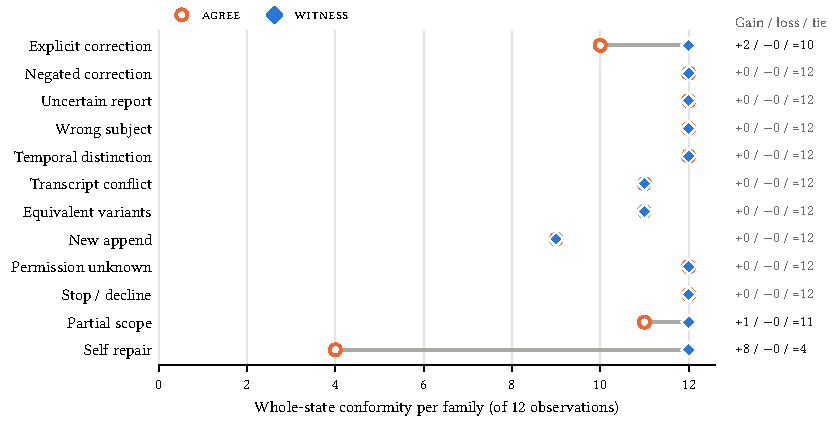
\includegraphics[width=\linewidth,height=.42\textheight,keepaspectratio]{media/figure_03.pdf}
\caption{Recovery by problem family on Gemini 2.5 Flash. The 11 observation-level gains of \witness{} over \agree{} come from five correction cases, and eight of them occur in self-repair.}\label{fig:A1}
\Description{Recovery by problem family on Gemini 2.5 Flash. The 11 observation-level gains come from five correction cases, and eight of them occur in self-repair.}
\end{figure}

\subsection{Statistics and Held Corrections}
The prespecified primary comparison is \witnessr{} minus \review{} on positive-change completion. Rates average the three repetitions within each eligible case, and the 95\% percentile interval uses 5,000 fixed-seed case-cluster bootstrap draws. The exact McNemar test first reduces each condition to a majority of three successes per case. The five planned model families keep their Holm accounting: three slots have observed tests (Gemini 2.5 Flash, Llama 3.1 8B, and Qwen3 14B), and the two uncollected slots (Online Appendix~C) enter with an adjustment value of one and no observed $p$. The \agree{}--\witness{} contrasts, family profiles, and failure counts are descriptive.

On Gemini 2.5 Flash, \agree{} held 11 required corrections that \witness{} admitted: all three repetitions of CT45 and CT46, two of CT01 and CT48, and one of CT42. Table~\ref{tab:A3} and Figure~\ref{fig:A1} show eight of them in the self-repair family. All reported runs are complete, and no failed output was regenerated. Five Gemini calls ended in rate-limit errors and lack token usage; the other 859 Gemini calls and all 864 Llama calls report usage.

\FloatBarrier
\setcounter{figure}{0}\setcounter{table}{0}
\renewcommand{\thefigure}{B\arabic{figure}}
\renewcommand{\thetable}{B\arabic{table}}
\section{Llama 3.1 8B and Eight-Configuration Profiles}
Llama 3.1 8B belonged to the original comparison and was not selected after its result. \agree{} and \witness{} each complete 0 of 33 strict corrections and 6 of 84 positive changes, against 29 for \review{}, 24 for \direct{}, and 25 for \refine{}. The \witnessr{}--\review{} case-mean difference is $-27.4$ percentage points (95\% case-cluster interval $-44.0$ to $-10.7$), with exact majority-case McNemar $p=.0117$ and original five-slot Holm-adjusted $p=.0586$. All 864 provider calls returned, but the controlled path produced 68 invalid final outputs out of 144, against one for \review{}, two for \direct{}, and none for \refine{}, and its valid outputs also contain action and state failures. Model family, size, four-bit quantization, runtime, and output-schema demands vary together in this configuration, so the result does not isolate parameter count.

Only two Llama outputs reach $H$. In CT47, repetition 1, \witness{} keeps a hold on an eligible correction that \allow{} releases. Overall, \allow{} produces one more reference-violating state than \agree{}, \literal{}, and \witness{} (25 versus 24), and strict correction completion remains zero under every rule (Table~\ref{tab:B1}). Table~\ref{tab:B2} sets the complete pipelines of the same eight configurations side by side; these pipelines generate different proposals.

\begin{table}[H]
\centering
\caption{Admission rules on identical proposals for the eight configurations of the original protocol and the Gemini series, in the order \agree{} / \allow{} / \literal{} / \witness{}. The Gemini rows repeat Table~6 of the main article. $H$ counts outputs that reach the held set.}\label{tab:B1}
\small
\setlength{\tabcolsep}{4pt}
\begin{tabular}{@{}lllr@{}}
\toprule
\textbf{Configuration} & \textbf{Correction /33} & \textbf{Viol. /144} & \textbf{$H$ outputs} \\
\midrule
Gemini 2.5 Flash & 22 / 33 / 33 / 33 & 3 / 3 / 3 / 3 & 11 \\
Gemini 2.5 Pro & 31 / 31 / 31 / 31 & 3 / 9 / 4 / 3 & 6 \\
Gemini 2.5 Flash-Lite & 31 / 31 / 31 / 31 & 16 / 19 / 16 / 16 & 3 \\
Gemini 3 Flash Preview & 33 / 33 / 33 / 33 & 12 / 12 / 12 / 12 & 0 \\
Gemini 3.1 Pro Preview & 33 / 33 / 33 / 33 & 2 / 2 / 2 / 2 & 0 \\
Gemini 3.5 Flash-Lite & 32 / 32 / 32 / 32 & 7 / 12 / 7 / 7 & 5 \\
Gemini 3.8 Flash & 33 / 33 / 33 / 33 & 1 / 1 / 1 / 1 & 0 \\
Llama 3.1 8B & 0 / 0 / 0 / 0 & 24 / 25 / 24 / 24 & 2 \\
\bottomrule
\end{tabular}
\end{table}

\begin{table}[H]
\centering
\caption{Complete pipelines for the same eight configurations, in the order \direct{} / \review{} / controlled path. Counts combine three repetitions within each configuration and are not pooled across configurations.}\label{tab:B2}
\small
\setlength{\tabcolsep}{4pt}
\begin{tabular}{@{}lll@{}}
\toprule
\textbf{Configuration} & \textbf{Correction /33} & \textbf{Viol. /144} \\
\midrule
Gemini 2.5 Flash & 32 / 33 / 33 & 6 / 5 / 3 \\
Gemini 2.5 Pro & 33 / 32 / 31 & 8 / 8 / 3 \\
Gemini 2.5 Flash-Lite & 33 / 33 / 31 & 14 / 14 / 16 \\
Gemini 3 Flash Preview & 33 / 33 / 33 & 6 / 6 / 12 \\
Gemini 3.1 Pro Preview & 33 / 33 / 33 & 3 / 3 / 2 \\
Gemini 3.5 Flash-Lite & 33 / 33 / 32 & 1 / 0 / 7 \\
Gemini 3.8 Flash & 33 / 33 / 33 & 1 / 0 / 1 \\
Llama 3.1 8B & 0 / 4 / 0 & 14 / 17 / 24 \\
\bottomrule
\end{tabular}
\end{table}

\FloatBarrier
\setcounter{figure}{0}\setcounter{table}{0}
\renewcommand{\thefigure}{C\arabic{figure}}
\renewcommand{\thetable}{C\arabic{table}}
\section{Model Roster, Generation Settings, and Resources}
\subsection{Roster}
The original protocol planned a Holm-adjusted primary comparison for five model families. Gemini 2.5 Flash, Llama 3.1 8B, and Qwen3 14B (local 4-bit) completed. EXAONE 3.5 7.8B stopped at the technical probe for incomplete coverage, and a planned 12B configuration was replaced before collection, so neither contributes a result (Table~\ref{tab:C1}). An earlier version of this analysis excluded the Qwen3 14B results after they had become available; they are reported in full here and in the main article, and the five-slot Holm accounting is the one fixed before collection. The later Gemini configurations reuse the 48 cases, are descriptive, and do not enter the Holm family. ``Complete'' means that every scheduled main-source call and the first analysis finished; a technical stop is not a zero score. Online Appendix~G records how the 21-configuration panel was selected.

\begin{table}[H]
\centering
\caption{Model roster of the original protocol and the Gemini series.}\label{tab:C1}
\small
\setlength{\tabcolsep}{4pt}
\begin{tabular}{@{}>{\raggedright\arraybackslash}p{\dimexpr0.50\linewidth-5.4pt\relax}>{\raggedright\arraybackslash}p{\dimexpr0.20\linewidth-5.4pt\relax}>{\raggedright\arraybackslash}p{\dimexpr0.30\linewidth-5.4pt\relax}@{}}
\toprule
\textbf{Model} & \textbf{Design block} & \textbf{Main-source status} \\
\midrule
Gemini 2.5 Flash & Original family & Complete \\
Llama 3.1 8B & Original family & Complete \\
Qwen3 14B (4-bit) & Original family & Complete \\
EXAONE 3.5 7.8B & Original family & Stopped at technical probe \\
Planned 12B configuration & Original family & Replaced before collection \\
Gemini 3.8 Flash & Later addition & Complete \\
Gemini 2.5 Pro, 2.5 Flash-Lite, 3 Flash Preview, 3.1 Pro Preview, 3.5 Flash-Lite & Gemini series & Complete \\
Gemini 3.5 Flash, 3.6 Flash, 3.7 Flash & Gemini series & Stopped by provider errors \\
Gemini 3.1 Flash-Lite & Gemini series & Stopped at technical probe \\
\bottomrule
\end{tabular}
\end{table}

The original call budget was $48\times3\times6=864$ main-source calls plus 12 technical probes per configuration; the later Gemini runs separately allowed 864 main-source, 96 contrast-set, and 12 probe calls, with no retry. These budgets are not effective sample sizes: every complete configuration shares the same 48 authored cases.

\subsection{Generation Settings}
Table~\ref{tab:C2} lists the requested settings for the seven Gemini configurations and Llama 3.1 8B. Requested temperature and thinking settings are not measurements of effective sampling, and returned cloud version strings identify service names rather than immutable weights.

\begin{table}[H]
\centering
\caption{Requested generation settings. Caps are maximum output tokens for ordinary stages / feedback. Thinking numbers are requested token budgets, and LOW is the requested thinking level. Version rows count calls whose returned version string matches the requested identifier.}\label{tab:C2}
\small
\setlength{\tabcolsep}{4pt}
\begin{tabular}{@{}lrrrr@{}}
\toprule
\textbf{Requested model identifier} & \textbf{Caps} & \textbf{Temperature} & \textbf{Thinking} & \textbf{Version rows} \\
\midrule
\texttt{gemini-2.5-flash} & 2048/512 & 0.2 & 0 & 859/864 \\
\texttt{gemini-2.5-pro} & 8192/2048 & 0.2 & 128 & 853/864 \\
\texttt{gemini-2.5-flash-lite} & 8192/2048 & 0.2 & 0 & 851/864 \\
\texttt{gemini-3-flash-preview} & 8192/2048 & 0.2 & LOW & 861/864 \\
\texttt{gemini-3.1-pro-preview} & 8192/2048 & 0.2 & LOW & 855/864 \\
\texttt{gemini-3.5-flash-lite} & 8192/2048 & provider default & LOW & 856/864 \\
\texttt{gemini-3.8-flash} & 8192/2048 & 0.2 & LOW & 864/864 \\
\texttt{Llama-3.1-8B-Instruct-4bit} & 2048/512 & 0.2 & -- & 864/864 \\
\bottomrule
\end{tabular}
\end{table}

Cloud calls used a REST adapter written in Python, and Llama 3.1 8B used MLX adapter code with a fixed runtime path; its adapter records the model identifier as the version rather than a version returned by a server.

\subsection{Recorded Resources}
Each configuration made 864 physical calls, including failures; across the eight configurations, 6,863 of 6,912 calls returned. Token usage is missing for the 49 failed calls, and summed latency is not elapsed study time (Table~\ref{tab:C3}). Table~\ref{tab:C4} isolates the two-call \review{} pipeline and the controlled path. \witness{} uses the same two saved calls per output as \agree{}, so evaluating it, like \allow{} and \literal{}, adds no model call.

\begin{table}[H]
\centering
\caption{Recorded physical calls for the seven Gemini configurations and Llama 3.1 8B. Token sums use the calls that report a value; reasoning tokens are reported separately where present. Latency is a sum of per-call seconds, not wall-clock time.}\label{tab:C3}
\footnotesize
\setlength{\tabcolsep}{4pt}
\begin{tabular}{@{}lrrrrrrr@{}}
\toprule
\textbf{Configuration} & \textbf{OK} & \textbf{Failed} & \textbf{Input} & \textbf{Output} & \textbf{Reasoning} & \textbf{Usage} & \textbf{$\sum$ s} \\
\midrule
Gemini 2.5 Flash & 859 & 5 & 1,546,070 & 189,292 & 0 & 859/864 & 1441.6 \\
Gemini 2.5 Pro & 853 & 11 & 1,542,438 & 201,837 & 76,052 & 853/864 & 3493.6 \\
Gemini 2.5 Flash-Lite & 851 & 13 & 1,575,962 & 230,385 & 0 & 851/864 & 1289.8 \\
Gemini 3 Flash Preview & 861 & 3 & 2,301,473 & 126,385 & 43,639 & 861/864 & 2804.3 \\
Gemini 3.1 Pro Preview & 855 & 9 & 2,267,984 & 170,045 & 27,803 & 855/864 & 3302.1 \\
Gemini 3.5 Flash-Lite & 856 & 8 & 2,273,983 & 146,597 & 0 & 856/864 & 1316.2 \\
Gemini 3.8 Flash & 864 & 0 & 2,294,575 & 115,377 & 2,271 & 864/864 & 3019.5 \\
Llama 3.1 8B & 864 & 0 & 1,570,636 & 161,305 & -- & 864/864 & 9408.9 \\
\bottomrule
\end{tabular}
\end{table}

\begin{table}[H]
\centering
\caption{Saved calls behind the \review{} pipeline and the controlled path. Each covers 144 outputs and 288 physical calls; these sums overlap with Table~\ref{tab:C3} and should not be added to it.}\label{tab:C4}
\small
\setlength{\tabcolsep}{4pt}
\begin{tabular}{@{}llrrrr@{}}
\toprule
\textbf{Configuration} & \textbf{Path} & \textbf{Calls} & \textbf{Input} & \textbf{Output} & \textbf{$\sum$ s} \\
\midrule
Gemini 2.5 Flash & \review{} & 288 & 512,062 & 54,918 & 431.9 \\
 & Controlled & 288 & 533,378 & 77,022 & 519.4 \\
Gemini 2.5 Pro & \review{} & 288 & 508,872 & 57,657 & 1088.7 \\
 & Controlled & 288 & 533,190 & 89,653 & 1302.2 \\
Gemini 2.5 Flash-Lite & \review{} & 288 & 509,749 & 58,254 & 378.7 \\
 & Controlled & 288 & 533,820 & 82,205 & 427.1 \\
Gemini 3 Flash Preview & \review{} & 288 & 821,829 & 40,476 & 877.7 \\
 & Controlled & 288 & 804,384 & 54,497 & 1093.1 \\
Gemini 3.1 Pro Preview & \review{} & 288 & 809,106 & 54,048 & 1082.7 \\
 & Controlled & 288 & 795,470 & 85,360 & 1197.4 \\
Gemini 3.5 Flash-Lite & \review{} & 288 & 817,567 & 43,449 & 417.2 \\
 & Controlled & 288 & 787,723 & 70,089 & 494.6 \\
Gemini 3.8 Flash & \review{} & 288 & 823,976 & 36,927 & 955.8 \\
 & Controlled & 288 & 801,856 & 57,104 & 1289.4 \\
Llama 3.1 8B & \review{} & 288 & 525,149 & 49,177 & 3030.1 \\
 & Controlled & 288 & 537,723 & 69,668 & 3635.4 \\
\bottomrule
\end{tabular}
\end{table}

\FloatBarrier
\setcounter{figure}{0}\setcounter{table}{0}
\renewcommand{\thefigure}{D\arabic{figure}}
\renewcommand{\thetable}{D\arabic{table}}
\section{Contrast Set}
The 24-case contrast set was written after the initial recovery finding by a separate source-writing agent that received the schema but neither the rule code nor earlier outputs. It pairs 12 supported and 12 unsupported edits with matched records and task instructions, and its references were written with AI assistance before execution. The set was run once on Gemini 2.5 Flash (Vertex, temperature 0.2, thinking budget 0, at most 2,048 output tokens, no retries). Case labels and expected states were withheld from model messages; branch order was counterbalanced by case identifier, and case order was shuffled with seed 2026092720. Each case used two extraction-and-proposal calls shared by the admission rules and two separate \review{} calls: 96 calls, 95 of which returned; one draft-stage rate-limit error was followed by the scheduled final call.

The admission rules received identical saved proposals, executed on isolated SQLite states initialized from the same case. All 24 extraction-and-proposal paths were valid, 18 cases contained a proposed CORRECT, and \agree{} held six for lack of shared support although every reading was validly covered. \witness{} restored five, each with affirmed, target-linked witnesses, and kept one hold because a witness was not affirmed; \literal{} and \allow{} restored all six. The scorer compares persistent record identifiers, subjects, relations, values, and time fields.

On supported cases, paired gains and losses are 5/0 for \witness{} versus \agree{}, 0/0 versus \allow{}, and 0/2 versus \review{}; on unsupported cases they are 0/0, 1/0, and 2/1. The corresponding exact McNemar $p$ values are .0625, 1, .5, 1, 1, and 1; with one draw per case and no multiplicity adjustment, they describe these cases only (Table~\ref{tab:D1}).

\begin{table}[H]
\centering
\caption{Whole-state outcomes on the contrast set with 95\% Wilson intervals; each stratum has 12 cases.}\label{tab:D1}
\small
\setlength{\tabcolsep}{4pt}
\begin{tabular}{@{}lll@{}}
\toprule
\textbf{Condition} & \textbf{Supported edit completed} & \textbf{Unsupported edit preserved} \\
\midrule
\agree{} & 5/12, 41.7\% [19.3, 68.0] & 9/12, 75.0\% [46.8, 91.1] \\
\allow{} & 10/12, 83.3\% [55.2, 95.3] & 8/12, 66.7\% [39.1, 86.2] \\
\literal{} & 10/12, 83.3\% [55.2, 95.3] & 8/12, 66.7\% [39.1, 86.2] \\
\witness{} & 10/12, 83.3\% [55.2, 95.3] & 9/12, 75.0\% [46.8, 91.1] \\
\review{} & 12/12, 100.0\% [75.8, 100.0] & 8/12, 66.7\% [39.1, 86.2] \\
\bottomrule
\end{tabular}
\end{table}

\begin{table}[H]
\centering
\caption{Translated trace of case N015, the only contrast-set case in which \witness{} and \allow{} differ. The two readings are alternatives for the same utterance, not two speakers.}\label{tab:D2}
\small
\setlength{\tabcolsep}{4pt}
\begin{tabular}{@{}>{\raggedright\arraybackslash}p{\dimexpr0.28\linewidth-4pt\relax}>{\raggedright\arraybackslash}p{\dimexpr0.72\linewidth-4pt\relax}@{}}
\toprule
\textbf{Stage} & \textbf{Saved content or executed result} \\
\midrule
Stored record & f1: participant, residence, Ulsan, present. \\
Task instruction & Edit only the current record. Add no other-person or other-time facts. Keep the record when the meaning is unresolved. \\
Reading 1 & I live in Changwon now. \\
Reading 2 & I do not live in Changwon now. \\
Shared proposal & CORRECT f1: residence $\leftarrow$ Changwon. \\
Shared reply & You live in Changwon. Understood. \\
Witnesses & Reading 1 affirmed; reading 2 negated. \\
\agree{} & Held for lack of shared support; Ulsan retained. \\
\witness{} & Hold kept because a witness is not affirmed; Ulsan retained. \\
\literal{} and \allow{} & Hold released; Changwon written. \\
\review{} & Changwon written from its separate proposal. \\
\bottomrule
\end{tabular}
\end{table}

The kept hold prevents the disputed overwrite, but the unchanged reply still asserts the disputed value, which separates protection of the stored state from the quality of the reply (Table~\ref{tab:D2}). The other unsupported-case failures of \witness{} and \allow{} keep the target but append facts outside the permitted edit scope. On supported cases, both rules replace all 12 target values, and two additional past-state records fail the whole-state endpoint.

\FloatBarrier
\setcounter{figure}{0}\setcounter{table}{0}
\renewcommand{\thefigure}{E\arabic{figure}}
\renewcommand{\thetable}{E\arabic{table}}
\section{Boundary Probe}
The 12-case boundary probe was run once with the same Gemini 2.5 Flash configuration and rule implementations, using 24 model calls and producing 36 condition rows rather than 36 cases. Its source and reference were written with AI assistance and fixed before collection. Six pairs share an initial record and vary whether the current utterance licenses updating it. Because no output reached $H$, all four admission rules produce the same state in every case (Table~\ref{tab:E1}).

\begin{table}[H]
\centering
\caption{Boundary-probe outcomes. A match requires a valid output and the complete expected fact map, so a correct target with an extra fact fails.}\label{tab:E1}
\small
\setlength{\tabcolsep}{4pt}
\begin{tabular}{@{}lll>{\raggedright\arraybackslash}p{0.42\linewidth}@{}}
\toprule
\textbf{Case} & \textbf{Expected edit} & \textbf{Boundary} & \textbf{Whole-state outcome (all rules)} \\
\midrule
W001 & Keep & Hypothetical & Match \\
W002 & Update & Speaker identity & Error: extra past address \\
W003 & Keep & Retracted certainty & Match \\
W004 & Update & Negation & Error: new hobby appended; retired target retained \\
W005 & Keep & Speaker identity & Match \\
W006 & Update & Quotation & Match \\
W007 & Keep & Negation & Match \\
W008 & Update & Retracted certainty & Match \\
W009 & Update & Hypothetical & Match \\
W010 & Keep & Quotation & Match \\
W011 & Update & Temporal scope & Match \\
W012 & Keep & Temporal scope & Error: extra past workplace \\
\bottomrule
\end{tabular}
\end{table}

For each rule, 4 of 6 supported edits (Wilson 95\% interval 30.0 to 90.3\%) and 5 of 6 unsupported edits (43.6 to 97.0\%) match the reference, and all 24 provider responses and 12 final outputs were valid. W004 shows a limit outside the held set. Both readings state that swimming is the current hobby and hiking has stopped; the proposal appends swimming and issues a CORRECT for hiking that keeps the old target. The hiking witness is negated, but \agree{} admits the old tuple because it is already stored, and since the operation is not a correction held for lack of support, \witness{} does not inspect it. In W007, one reading omits a negation about swimming while both continue to support the stored hiking record, and every rule keeps that record.

\FloatBarrier
\setcounter{figure}{0}\setcounter{table}{0}
\renewcommand{\thefigure}{F\arabic{figure}}
\renewcommand{\thetable}{F\arabic{table}}
\section{Public Task-Dialogue Probe}
The source contains 16 selected written user turns from MultiWOZ~2.4, paired with prior task-state subsets. The Gemini 2.5 Flash collection has 96 requests and 144 condition records across nine conditions; a planned run with a second model was dropped before this source was first scored. The reference and eligibility were fixed before collection: 10 same-task self-repairs are eligible, and six plan-change or annotation-ambiguous cases have no automatic correctness label. The reference adapts the dataset's state annotation and is not a new human assessment.

Focal agreement requires exactly one fact for each evaluated subject and relation, equal to the adapted annotation after case folding and whitespace normalization. Unlike positive-change completion, it does not require an allowed action, and generation validity is tracked separately; in the one provider-error case, the unchanged initial value differs from the reference and fails focal agreement.

\begin{table}[H]
\centering
\caption{Focal-state agreement on the 10 eligible self-repairs. The reply-rendered variants of \agree{} and \witness{} have the same states as \agree{} and \witness{}.}\label{tab:F1}
\small
\setlength{\tabcolsep}{5pt}
\begin{tabular}{@{}lrrrrrrr@{}}
\toprule
 & \textbf{\direct{}} & \textbf{\review{}} & \textbf{\refine{}} & \textbf{\agree{}} & \textbf{\allow{}} & \textbf{\literal{}} & \textbf{\witness{}} \\
\midrule
Agreement /10 & 10 & 10 & 5 & 3 & 7 & 4 & 4 \\
\bottomrule
\end{tabular}
\end{table}

\direct{} and \review{} produce identical final states on every source case, as do \witness{} and \literal{}. \agree{} holds eight corrections and one append; \witness{} and \literal{} restore four of the held corrections, and \allow{} restores all eight. One \witness{} restoration adds an eligible exact agreement, and \allow{} adds three more (Table~\ref{tab:F1}). A source spelling ``Thursday'' against a proposed ``thursday'' shows the cost of literal matching (main article, Section~6.4). In that saved example, the extracted fact list is empty, so normalizing existing facts cannot repair the hold; a lexical diagnostic that applies Unicode NFC, case folding, and whitespace normalization turns the value-to-source and value-to-quotation containment checks from false to true, but that repair was not executed or scored. One candidate-final rate-limit error yields six invalid records across the admission-rule conditions, and two other cases per admission-rule condition contain writes rejected by the executor; no failed request was retried. The source is written task dialogue, not noisy acoustic transcription or personal biography.

\FloatBarrier
\setcounter{figure}{0}\setcounter{table}{0}
\renewcommand{\thefigure}{G\arabic{figure}}
\renewcommand{\thetable}{G\arabic{table}}
\section{Complete Three Repetition Model Panel}
The main panel is selected from 28 configurations with 48 complete case triplets. Seven do not meet the common 95\% final-output-validity criterion and six additional archived configurations have incomplete triplets. Table~\ref{tab:J1} lists all 21 selected configurations, and Figure~\ref{fig:G1} plots their complete-pipeline differences. The eligibility criterion applies to each whole path over 144 observations; observed invalid outputs remain in the endpoint denominators. Table~\ref{tab:J2} records the remaining configuration coverage without interpreting uncollected episodes as zero-valued semantic outcomes.

The case-majority McNemar result for Gemini 2.5 Flash \agree{} versus \witness{} is $p=.125$, with four discordant cases, and is descriptive. The McNemar test concerns the binarized case-level outcome, whereas the effect size and case-cluster interval in Section~6.1 describe the mean difference. For the original whole-path primary comparison, the case-majority result is $p=1.00$. The expanded panel is exploratory, and its pointwise intervals do not supply a simultaneous model ranking. Missing pooled intervals remain marked rather than being constructed by combining intervals from different collection phases. Per repetition, the direction of the positive-completion difference changes on 11 of the 21 configurations, counting a tie as a direction (Table~\ref{tab:J4}), and strict correction completion under the controlled path matches \review{} on 17 configurations and is lower on 4.

\begin{table}[H]
\centering
\caption{All 21 complete configurations, \review{} \ensuremath{\rightarrow} controlled path. Every result combines three repetitions. Positive differences use 28 case clusters. A dash denotes an unavailable matching pooled interval; a partial-collection interval is never substituted.}\label{tab:J1}
\small
\setlength{\tabcolsep}{3pt}
\begin{tabular}{@{}>{\raggedright\arraybackslash}p{\dimexpr0.3182\linewidth-7.64pt\relax}>{\raggedright\arraybackslash}p{\dimexpr0.1364\linewidth-3.27pt\relax}>{\raggedright\arraybackslash}p{\dimexpr0.1364\linewidth-3.27pt\relax}>{\raggedright\arraybackslash}p{\dimexpr0.1364\linewidth-3.27pt\relax}>{\raggedright\arraybackslash}p{\dimexpr0.2727\linewidth-6.55pt\relax}@{}}
\toprule
\textbf{Configuration} & \textbf{Positive /84} & \textbf{Viol. /144} & \textbf{Invalid /144} & \textbf{Positive \ensuremath{\Delta} pp [95\% CI]} \\
\midrule
Claude Opus 4.5 & 79 \ensuremath{\rightarrow} 78 & 5 \ensuremath{\rightarrow} 6 & 0 \ensuremath{\rightarrow} 0 & -1.2 [-10.7, +4.8] \\
Claude Opus 4.6 & 76 \ensuremath{\rightarrow} 78 & 8 \ensuremath{\rightarrow} 6 & 3 \ensuremath{\rightarrow} 0 & +2.4 [-3.6, +10.7] \\
Claude Opus 4.7 & 78 \ensuremath{\rightarrow} 80 & 6 \ensuremath{\rightarrow} 3 & 0 \ensuremath{\rightarrow} 0 & +2.4 [-3.6, +9.5] \\
Claude Opus 4.8 & 81 \ensuremath{\rightarrow} 82 & 3 \ensuremath{\rightarrow} 2 & 0 \ensuremath{\rightarrow} 0 & +1.2 [+0.0, +3.6] \\
Claude Opus 5.5 & 69 \ensuremath{\rightarrow} 72 & 15 \ensuremath{\rightarrow} 12 & 0 \ensuremath{\rightarrow} 0 & +3.6 [+0.0, +9.5] \\
Claude Sonnet 4 & 77 \ensuremath{\rightarrow} 76 & 6 \ensuremath{\rightarrow} 6 & 4 \ensuremath{\rightarrow} 4 & -1.2 [-9.5, +7.1] \\
Claude Sonnet 4.5 & 79 \ensuremath{\rightarrow} 81 & 9 \ensuremath{\rightarrow} 3 & 0 \ensuremath{\rightarrow} 1 & +2.4 [+0.0, +6.0] \\
Claude Sonnet 4.6 & 81 \ensuremath{\rightarrow} 81 & 3 \ensuremath{\rightarrow} 3 & 2 \ensuremath{\rightarrow} 0 & +0.0 [+0.0, +0.0] \\
DeepSeek 3.2 & 81 \ensuremath{\rightarrow} 76 & 5 \ensuremath{\rightarrow} 7 & 2 \ensuremath{\rightarrow} 2 & -6.0 [-14.3, +0.0] \\
Gemini 2.5 Flash-Lite & 69 \ensuremath{\rightarrow} 56 & 14 \ensuremath{\rightarrow} 16 & 1 \ensuremath{\rightarrow} 4 & -15.5 [-34.5, +4.8] \\
Gemini 2.5 Pro & 71 \ensuremath{\rightarrow} 73 & 8 \ensuremath{\rightarrow} 3 & 3 \ensuremath{\rightarrow} 3 & +2.4 [-8.3, +11.9] \\
Gemini 3.1 Pro Preview & 81 \ensuremath{\rightarrow} 81 & 3 \ensuremath{\rightarrow} 2 & 3 \ensuremath{\rightarrow} 2 & +0.0 [-3.6, +3.6] \\
Gemini 3.5 Flash-Lite & 84 \ensuremath{\rightarrow} 74 & 0 \ensuremath{\rightarrow} 7 & 1 \ensuremath{\rightarrow} 5 & -11.9 [-23.8, -2.4] \\
Gemini 3.8 Flash & 84 \ensuremath{\rightarrow} 83 & 0 \ensuremath{\rightarrow} 1 & 0 \ensuremath{\rightarrow} 0 & -1.2 [-3.6, +0.0] \\
Gemini 3 Flash Preview & 78 \ensuremath{\rightarrow} 71 & 6 \ensuremath{\rightarrow} 12 & 1 \ensuremath{\rightarrow} 0 & -8.3 [-19.0, +0.0] \\
Gemini 2.5 Flash & 82 \ensuremath{\rightarrow} 80 & 5 \ensuremath{\rightarrow} 3 & 1 \ensuremath{\rightarrow} 1 & -2.4 [-6.0, +0.0] \\
GLM 5 & 81 \ensuremath{\rightarrow} 81 & 3 \ensuremath{\rightarrow} 2 & 0 \ensuremath{\rightarrow} 0 & +0.0 [-3.6, +3.6] \\
GPT 5.6 Luna & 77 \ensuremath{\rightarrow} 80 & 7 \ensuremath{\rightarrow} 4 & 0 \ensuremath{\rightarrow} 0 & +3.6 [---] \\
GPT 5.6 Sol & 71 \ensuremath{\rightarrow} 75 & 13 \ensuremath{\rightarrow} 8 & 0 \ensuremath{\rightarrow} 0 & +4.8 [+0.0, +10.7] \\
GPT 5.6 Terra & 71 \ensuremath{\rightarrow} 76 & 13 \ensuremath{\rightarrow} 5 & 0 \ensuremath{\rightarrow} 1 & +6.0 [-1.2, +15.5] \\
Qwen3 14B (4-bit) & 73 \ensuremath{\rightarrow} 66 & 14 \ensuremath{\rightarrow} 20 & 0 \ensuremath{\rightarrow} 0 & -8.3 [-23.8, +6.0] \\
\bottomrule
\end{tabular}
\end{table}
\begin{figure}[H]
\centering
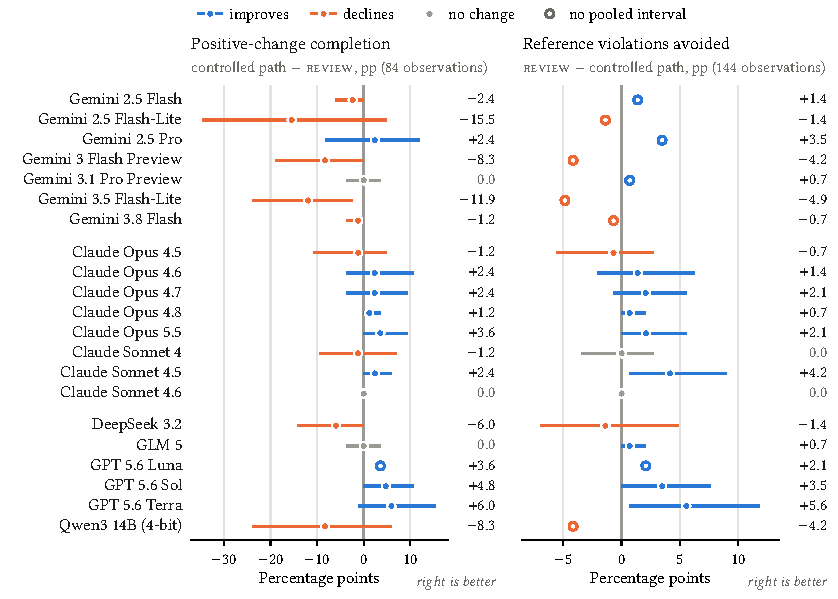
\includegraphics[width=\linewidth,height=.62\textheight,keepaspectratio]{media/figure_06.pdf}
\caption{Effects of the complete pipelines on the same 48 cases over three repetitions, oriented so that improvement is to the right (more positive completions and fewer reference-violating states). Positive completion uses 84 observations from 28 cases, and the reference-violation endpoint uses 144 observations from 48 cases. Blue marks improvement, orange decline, and gray no change; values at the right are point estimates in percentage points. Lines show the matching archived pointwise 95\% case-cluster intervals, and open points mark configurations without a complete pooled interval.}\label{fig:G1}
\Description{Effects of the complete pipelines on the same 48 cases over three repetitions, oriented so that improvement is to the right: more positive completions and fewer reference-violating states. Lines are pointwise 95 percent case-cluster intervals; open points mark configurations without a complete pooled interval.}
\end{figure}
\begin{table}[H]
\centering
\caption{Configuration selection record. All thresholds are technical and use the same rule for both paths.}\label{tab:J2}
\small
\setlength{\tabcolsep}{3pt}
\begin{tabular}{@{}>{\raggedright\arraybackslash}p{\dimexpr0.3485\linewidth-6.27pt\relax}>{\raggedright\arraybackslash}p{\dimexpr0.1515\linewidth-2.73pt\relax}>{\raggedright\arraybackslash}p{\dimexpr0.1818\linewidth-3.27pt\relax}>{\raggedright\arraybackslash}p{\dimexpr0.3182\linewidth-5.73pt\relax}@{}}
\toprule
\textbf{Configuration} & \textbf{Complete cases per repetition} & \textbf{Valid \review{} / controlled} & \textbf{Reason outside main panel} \\
\midrule
Claude Haiku 4.5 & 48 / 48 / 48 & 115/144; 96/144 & Below 95\% valid final outputs \\
Claude Opus 5 & 23 / 0 / 0 & Incomplete & Fewer than 48 complete case triplets \\
Claude Sonnet 5 & 48 / 46 / 0 & Incomplete & Fewer than 48 complete case triplets \\
EXAONE 4 32B & 48 / 48 / 48 & 136/144; 123/144 & Below 95\% valid final outputs \\
Llama 3.1 8B & 48 / 48 / 48 & 143/144; 76/144 & Below 95\% valid final outputs \\
MiniMax M2.1 & 48 / 3 / 0 & Incomplete & Fewer than 48 complete case triplets \\
MiniMax M2.5 & 48 / 40 / 0 & Incomplete & Fewer than 48 complete case triplets \\
Qwen2.5 7B Instruct & 48 / 48 / 48 & 87/144; 72/144 & Below 95\% valid final outputs \\
Qwen2.5 32B & 48 / 48 / 48 & 141/144; 123/144 & Below 95\% valid final outputs \\
Qwen3 32B & 48 / 48 / 48 & 141/144; 136/144 & Below 95\% valid final outputs \\
Qwen3 4B Instruct 2507 & 48 / 48 / 48 & 30/144; 51/144 & Below 95\% valid final outputs \\
Qwen3 8B & 25 / 0 / 0 & Incomplete & Fewer than 48 complete case triplets \\
Qwen3 Coder Next & 48 / 25 / 0 & Incomplete & Fewer than 48 complete case triplets \\
\bottomrule
\end{tabular}
\end{table}
\begin{table}[H]
\centering
\caption{Sensitivity to final-output validity among configurations with all three repetitions complete. These descriptive counts do not select a threshold for the most favorable result.}\label{tab:J3}
\small
\setlength{\tabcolsep}{3pt}
\begin{tabular}{@{}>{\raggedright\arraybackslash}p{\dimexpr0.1970\linewidth-3.55pt\relax}>{\raggedright\arraybackslash}p{\dimexpr0.1515\linewidth-2.73pt\relax}>{\raggedright\arraybackslash}p{\dimexpr0.3258\linewidth-5.86pt\relax}>{\raggedright\arraybackslash}p{\dimexpr0.3258\linewidth-5.86pt\relax}@{}}
\toprule
\textbf{Minimum validity} & \textbf{Configu\-rations} & \textbf{Positive higher / lower / same} & \textbf{Reference violations lower / higher / same} \\
\midrule
100\% & 9 & 5 / 3 / 1 & 6 / 3 / 0 \\
95\% & 21 & 9 / 9 / 3 & 12 / 7 / 2 \\
90\% & 22 & 9 / 10 / 3 & 12 / 8 / 2 \\
No validity filter & 28 & 10 / 15 / 3 & 16 / 10 / 2 \\
\bottomrule
\end{tabular}
\end{table}
\begin{table}[H]
\centering
\caption{Within-panel repetition stability on the same 21 configurations. All main outcome tables use the three-repetition pooled estimates.}\label{tab:J4}
\small
\setlength{\tabcolsep}{3pt}
\begin{tabular}{@{}>{\raggedright\arraybackslash}p{\dimexpr0.1667\linewidth-4.00pt\relax}>{\raggedright\arraybackslash}p{\dimexpr0.1818\linewidth-4.36pt\relax}>{\raggedright\arraybackslash}p{\dimexpr0.2197\linewidth-5.27pt\relax}>{\raggedright\arraybackslash}p{\dimexpr0.2197\linewidth-5.27pt\relax}>{\raggedright\arraybackslash}p{\dimexpr0.2121\linewidth-5.09pt\relax}@{}}
\toprule
\textbf{Repetition} & \textbf{Configu\-rations} & \textbf{Positive higher} & \textbf{Positive lower} & \textbf{Same} \\
\midrule
1 & 21 & 7 & 8 & 6 \\
2 & 21 & 6 & 7 & 8 \\
3 & 21 & 7 & 7 & 7 \\
\bottomrule
\end{tabular}
\end{table}

\subsection{Exposure of Controlled-Path Proposals on All 21 Configurations}
Table~\ref{tab:J5} extends the exposure count of Section~6.2 from the seven Gemini configurations to the whole panel. For every configuration, \agree{} and \witness{} are the saved conditions on the controlled-path proposals, and \literal{} is the exact replay executed with the frozen executor as the comparator for normalized \literal{} (Section~6.4); all three use the same extraction and proposal in each configuration, case, and repetition. An output is exposed when \agree{} holds at least one proposed CORRECT for lack of shared extracted support while every reading is validly covered. The counts come from the saved gate logs; no output was regenerated or rescored. \allow{} was replayed only for the Gemini configurations (Table~6) and Qwen3 14B (Section~6.2), so its column is omitted.

\begin{table}[H]
\centering
\caption{Controlled-path exposure on the 21 panel configurations. ``Released'' counts exposed outputs whose held correction both evidence checks restore; every such release completes a required correction. ``\literal{} only'' counts releases by \literal{} that \witness{} holds; both produce a reference-violating state. ``Kept'' counts holds that all three rules keep; all 35 lie in cases that require no change, and the held state conforms to the reference in each. The last two columns are in the order \agree{} / \literal{} / \witness{} and combine three repetitions; the panel totals use 693 correction and 3,024 all-case observations.}\label{tab:J5}
\small
\setlength{\tabcolsep}{3pt}
\begin{tabular}{@{}>{\raggedright\arraybackslash}p{\dimexpr0.2500\linewidth-6pt\relax}>{\raggedright\arraybackslash}p{\dimexpr0.2300\linewidth-6pt\relax}rrr>{\raggedright\arraybackslash}p{\dimexpr0.1300\linewidth-6pt\relax}>{\raggedright\arraybackslash}p{\dimexpr0.1300\linewidth-6pt\relax}@{}}
\toprule
\textbf{Configuration} & \textbf{$H$ outputs (cases)} & \textbf{Rel.} & \textbf{\literal{} only} & \textbf{Kept} & \textbf{Correction /33} & \textbf{Viol. /144} \\
\midrule
Claude Sonnet 4 & 3 (CT21) & 0 & 0 & 3 & 31/31/31 & 6/6/6 \\
Claude Sonnet 4.5 & 4 (CT21, CT22) & 0 & 0 & 4 & 33/33/33 & 3/3/3 \\
DeepSeek 3.2 & 4 (CT21, CT22, CT46) & 1 & 0 & 3 & 32/33/33 & 7/7/7 \\
Gemini 2.5 Flash & 11 (CT01, CT42, CT45, CT46, CT48) & 11 & 0 & 0 & 22/33/33 & 3/3/3 \\
Gemini 2.5 Flash-Lite & 3 (CT21) & 0 & 0 & 3 & 31/31/31 & 16/16/16 \\
Gemini 2.5 Pro & 6 (CT15, CT21, CT22) & 0 & 1 & 5 & 31/31/31 & 3/4/3 \\
Gemini 3.5 Flash-Lite & 5 (CT21, CT22) & 0 & 0 & 5 & 32/32/32 & 7/7/7 \\
GLM 5 & 3 (CT11, CT21, CT22) & 0 & 1 & 2 & 33/33/33 & 2/3/2 \\
Qwen3 14B (4-bit) & 10 (CT21, CT24, CT39, CT40) & 0 & 0 & 10 & 33/33/33 & 20/20/20 \\
\addlinespace[2pt]
12 other configurations & 0 & -- & -- & -- & equal & equal \\
\addlinespace[2pt]
All 21 & 49 (12 cases) & 12 & 2 & 35 & 673/685/685 & 131/133/131 \\
\bottomrule
\end{tabular}
\end{table}

The unexposed configurations are Claude Opus 4.5, 4.6, 4.7, 4.8, and 5.5, Claude Sonnet 4.6, Gemini 3 Flash Preview, 3.1 Pro Preview, and 3.8 Flash, and GPT 5.6 Luna, Sol, and Terra; on each, the three rules produce identical states. The 35 kept holds are 29 in the transcript-conflict cases CT21, CT22, and CT24 and six in the stop-or-decline cases CT39 and CT40. The two \literal{}-only releases are the Gemini 2.5 Pro workplace overwrite of Section~6.3 (CT15, repetition 2) and a GLM 5 destination overwrite (CT11, repetition 1) that replaces the stored value although the participant asked not to change it; the same case produces the witness-only hold on saved Qwen3 14B \review{} proposals (Section~6.4).
\FloatBarrier
\setcounter{figure}{0}\setcounter{table}{0}
\renewcommand{\thefigure}{H\arabic{figure}}
\renewcommand{\thetable}{H\arabic{table}}
\section{Detailed Translated Memory Examples}
\begin{figure}[H]
\centering
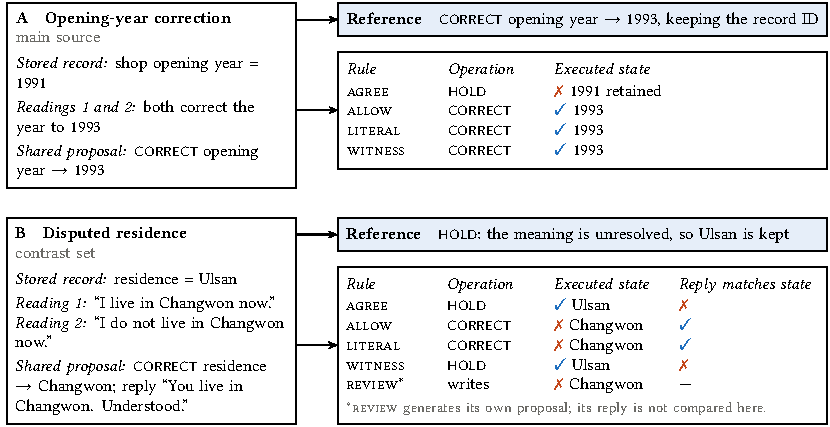
\includegraphics[width=\linewidth,height=.58\textheight,keepaspectratio]{media/figure_08.pdf}
\caption{Detailed translated examples. A shows the supported opening-year correction. B shows why a residence value appearing in both readings can still lack affirmative support when one reading negates it. The latter belongs to the separate contrast source.}\label{fig:K1}
\Description{Detailed translated examples. A shows the supported opening-year correction. B shows why a residence value appearing in both readings can still lack affirmative support when one reading negates it. The latter belongs to the separate contrast source.}
\end{figure}
\begin{figure}[H]
\centering
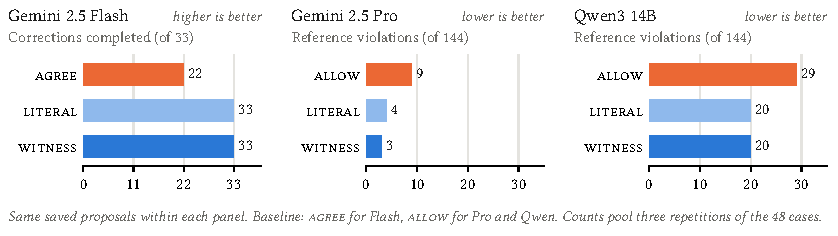
\includegraphics[width=\linewidth,height=.5\textheight,keepaspectratio]{media/figure_04.pdf}
\caption{Three component changes on fixed proposals. Gemini 2.5 Flash retains more correct corrections, Gemini 2.5 Pro admits fewer updates that violate the reference, and Qwen3 14B also reduces reference violations. Denominators and baselines differ as labeled; all panels are component comparisons.}\label{fig:K2}
\Description{Three component changes on fixed proposals. Gemini 2.5 Flash retains more correct corrections, Gemini 2.5 Pro admits fewer updates that violate the reference, and Qwen3 14B also reduces reference violations.}
\end{figure}
\FloatBarrier
\setcounter{figure}{0}\setcounter{table}{0}
\renewcommand{\thefigure}{I\arabic{figure}}
\renewcommand{\thetable}{I\arabic{table}}
\section{Admission Bounds, Operation Split, and Variant Audit on Saved Review Proposals}
This appendix completes the \review{}+gate replay of Section~6.4 with its two bounds, \review{}+\agree{} and \review{}+\allow{}, and separates the gate's APPEND and CORRECT decisions. All five conditions use the same saved \review{} proposals and the extractions from the same configuration, case and repetition (21 configurations $\times$ 48 cases $\times$ 3 repetitions). The two bounds were added after the \literal{} and \witness{} hybrids had been inspected. They apply the original rule definitions with the frozen executor and were scored once with the archived evaluator and reference: 6,048 new condition outputs, no model or provider call, no recomputation of the saved \review{}, \review{}+\literal{} or \review{}+\witness{} scores, and no change in the hashes of the frozen source files. The comparison is retrospective and reuses the authored cases; it adds no independent situations and no human judgment of the outputs.

Figure~\ref{fig:I0} summarizes the five conditions, and Table~\ref{tab:L1} restates how each condition treats the two operations. Tables~\ref{tab:L2}--\ref{tab:L4} give the endpoint totals, the decision counts by operation, and the attribution of paired changes; Table~\ref{tab:L5} splits the totals by the reference-defined case strata, Table~\ref{tab:L6} gives pooled paired intervals, and Table~\ref{tab:L7} lists the only five configurations on which the four rules differ. Table~\ref{tab:L8} and Figure~\ref{fig:L1} keep the per-configuration \review{}$\rightarrow$\review{}+\witness{} results. Table~\ref{tab:L9} audits which of the 82 avoided reference violations are variants of a required fact.

\begin{figure}[H]
\centering
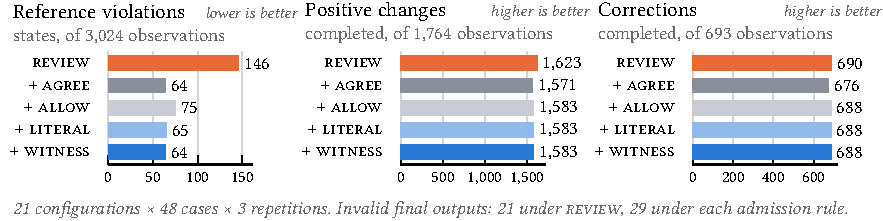
\includegraphics[width=\linewidth,height=.40\textheight,keepaspectratio]{media/figure_07.pdf}
\caption{Admission applied to saved \review{} proposals: the \agree{} and \allow{} bounds and the two evidence checks. The reference-violation endpoint follows the fixed state reference, including exact tuple mismatches. The same 21 configurations and all three repetitions appear in every bar; denominators are 3,024 for reference violations, 1,764 for positive changes, and 693 for corrections. Table~\ref{tab:L8} and Figure~\ref{fig:L1} report every configuration.}\label{fig:I0}
\Description{Admission applied to saved Review proposals. Reference violations fall from 146 to 64 with Agree, 75 with Allow, 65 with Literal, and 64 with Witness; successful positive changes fall from 1,623 to 1,571 with Agree and 1,583 with the other rules; successful corrections fall from 690 to 676 with Agree and 688 with the other rules.}
\end{figure}

\begin{table}[H]
\centering
\caption{Conditions on the same saved \review{} proposal. Extraction coverage, retention permission and the executor's checks are shared; an invalid extraction leaves the initial state and counts as an invalid output.}\label{tab:L1}
\small
\setlength{\tabcolsep}{3pt}
\begin{tabular}{@{}>{\raggedright\arraybackslash}p{\dimexpr0.2200\linewidth-2.64pt\relax}>{\raggedright\arraybackslash}p{\dimexpr0.3400\linewidth-4.08pt\relax}>{\raggedright\arraybackslash}p{\dimexpr0.4400\linewidth-5.28pt\relax}@{}}
\toprule
\textbf{Condition} & \textbf{APPEND} & \textbf{CORRECT} \\
\midrule
\review{} & No gate; executor checks only. & No gate; executor checks only. \\
\review{} + \agree{} & Held unless the tuple is supported by every reading's fact list or already stored. & Same test as APPEND; held corrections form $H$ when every reading is validly covered. \\
\review{} + \allow{} & As \agree{}. & Restores every correction in $H$. \\
\review{} + \literal{} & As \agree{}. & Restores a correction in $H$ when $L_j=1$ (Section~4.1). \\
\review{} + \witness{} & As \agree{}. & Restores a correction in $H$ when $W_j=1$ (Section~4.1). \\
\bottomrule
\end{tabular}
\end{table}

\begin{table}[H]
\centering
\caption{Endpoint totals on saved \review{} proposals. The first five columns use all 3,024 observations (positive changes 1,764; corrections 693). The last three columns restrict all conditions to the 2,995 observations whose \review{} output and extraction are both valid, so that invalid extractions do not enter the comparison.}\label{tab:L2}
\small
\setlength{\tabcolsep}{3pt}
\begin{tabular}{@{}lrrrrr@{\hspace{9pt}}rrr@{}}
\toprule
 & \multicolumn{5}{c}{\textbf{All observations}} & \multicolumn{3}{c}{\textbf{Valid in every condition}} \\
\cmidrule(lr){2-6}\cmidrule(l){7-9}
\textbf{Condition} & \textbf{Viol.\,$\downarrow$} & \textbf{Positive} & \textbf{Correct.} & \textbf{Invalid} & \textbf{Conform.} & \textbf{Viol.\,$\downarrow$} & \textbf{Positive} & \textbf{Correct.} \\
\midrule
\review{} & 146 & 1,623 & 690 & 21 & 2,849 & 146 & 1,619 & 688 \\
\review{} + \agree{} & 64 & 1,571 & 676 & 29 & 2,810 & 64 & 1,571 & 676 \\
\review{} + \allow{} & 75 & 1,583 & 688 & 29 & 2,811 & 75 & 1,583 & 688 \\
\review{} + \literal{} & 65 & 1,583 & 688 & 29 & 2,821 & 65 & 1,583 & 688 \\
\review{} + \witness{} & 64 & 1,583 & 688 & 29 & 2,822 & 64 & 1,583 & 688 \\
\bottomrule
\end{tabular}
\end{table}

\begin{table}[H]
\centering
\caption{Original \review{} decisions by operation. The unit is an operation decision, and one observation can contain several; these counts are therefore not added to the observation-level totals of Table~\ref{tab:L2}. ``Unavailable'' marks decisions in observations whose extraction was invalid. The last column counts executed operations that the reference marks as violating. \review{} has no gate, and in every condition 19 admitted appends were not executed by the shared executor.}\label{tab:L3}
\small
\setlength{\tabcolsep}{3pt}
\begin{tabular}{@{}llrrrrrr@{}}
\toprule
\textbf{Condition} & \textbf{Operation} & \textbf{Proposed} & \textbf{Admitted} & \textbf{Held} & \textbf{Unavail.} & \textbf{Executed} & \textbf{Exec.\ viol.} \\
\midrule
\review{} & APPEND & 1,087 & -- & -- & -- & 1,068 & 132 \\
 & CORRECT & 762 & -- & -- & -- & 762 & 14 \\
\addlinespace[2pt]
\review{} + \agree{} & APPEND & 1,087 & 977 & 108 & 2 & 958 & 61 \\
 & CORRECT & 762 & 737 & 23 & 2 & 737 & 3 \\
\addlinespace[2pt]
\review{} + \allow{} & APPEND & 1,087 & 977 & 108 & 2 & 958 & 61 \\
 & CORRECT & 762 & 760 & 0 & 2 & 760 & 14 \\
\addlinespace[2pt]
\review{} + \literal{} & APPEND & 1,087 & 977 & 108 & 2 & 958 & 61 \\
 & CORRECT & 762 & 750 & 10 & 2 & 750 & 4 \\
\addlinespace[2pt]
\review{} + \witness{} & APPEND & 1,087 & 977 & 108 & 2 & 958 & 61 \\
 & CORRECT & 762 & 749 & 11 & 2 & 749 & 3 \\
\bottomrule
\end{tabular}
\end{table}

\begin{table}[H]
\centering
\caption{Paired endpoint changes relative to \review{}, attributed to the operation whose gate decision differed in the same configuration, case and repetition; ``Inv.'' marks an invalid extraction. Relative to \review{}, no condition introduced a new reference violation or completed an additional positive change or correction, and no observation changed both operations. The attribution is descriptive and not an additive causal decomposition.}\label{tab:L4}
\small
\setlength{\tabcolsep}{3pt}
\begin{tabular}{@{}lrrr@{\hspace{8pt}}rrrr@{\hspace{8pt}}rrr@{}}
\toprule
 & \multicolumn{3}{c}{\textbf{Viol.\ prevented}} & \multicolumn{4}{c}{\textbf{Positive changes lost}} & \multicolumn{3}{c}{\textbf{Corrections lost}} \\
\cmidrule(lr){2-4}\cmidrule(lr){5-8}\cmidrule(l){9-11}
\textbf{Condition} & \textbf{APP.} & \textbf{COR.} & \textbf{All} & \textbf{APP.} & \textbf{COR.} & \textbf{Inv.} & \textbf{All} & \textbf{COR.} & \textbf{Inv.} & \textbf{All} \\
\midrule
\review{} + \agree{} & 71 & 11 & 82 & 36 & 12 & 4 & 52 & 12 & 2 & 14 \\
\review{} + \allow{} & 71 & 0 & 71 & 36 & 0 & 4 & 40 & 0 & 2 & 2 \\
\review{} + \literal{} & 71 & 10 & 81 & 36 & 0 & 4 & 40 & 0 & 2 & 2 \\
\review{} + \witness{} & 71 & 11 & 82 & 36 & 0 & 4 & 40 & 0 & 2 & 2 \\
\bottomrule
\end{tabular}
\end{table}

Between the rules, every paired difference involves CORRECT only. \review{}+\allow{}, +\literal{} and +\witness{} each complete 12 more corrections and positive changes than \review{}+\agree{}; \review{}+\allow{} has 11 more reference-violating states than \review{}+\agree{} and \review{}+\witness{}, and 10 more than \review{}+\literal{}. Of the 23 corrections that \agree{} holds, \allow{} releases 23 (11 executed with a reference violation), \literal{} 13 (one) and \witness{} 12 (none); the 12 releases shared by all three rules are the ones that complete a required correction. In every observation, the four rules make the same APPEND decisions.

\begin{table}[H]
\centering
\caption{Outcomes by case stratum (cases; observations). The strata come from the frozen reference and were not inferred from model outputs: the 11 correction-eligible cases of the strict-correction endpoint, the other 17 positive cases, which require new information, and the 20 cases that require no positive change.}\label{tab:L5}
\small
\setlength{\tabcolsep}{3pt}
\begin{tabular}{@{}llrrrrr@{}}
\toprule
\textbf{Stratum} & \textbf{Endpoint} & \textbf{\review{}} & \textbf{+\,\agree{}} & \textbf{+\,\allow{}} & \textbf{+\,\literal{}} & \textbf{+\,\witness{}} \\
\midrule
Correction-eligible (11; 693) & Viol. & 0 & 0 & 0 & 0 & 0 \\
 & Correction & 690 & 676 & 688 & 688 & 688 \\
 & Invalid & 3 & 5 & 5 & 5 & 5 \\
\addlinespace[2pt]
New-information (17; 1,071) & Viol. & 125 & 61 & 61 & 61 & 61 \\
 & Positive & 933 & 895 & 895 & 895 & 895 \\
 & Invalid & 2 & 4 & 4 & 4 & 4 \\
\addlinespace[2pt]
No change required (20; 1,260) & Viol. & 21 & 3 & 14 & 4 & 3 \\
 & Conformity & 1,223 & 1,237 & 1,226 & 1,236 & 1,237 \\
 & Invalid & 16 & 20 & 20 & 20 & 20 \\
\bottomrule
\end{tabular}
\end{table}

No condition produces a reference-violating state on the correction-eligible cases. On the new-information cases, the four rules coincide, and every reduction relative to \review{} (125 to 61) comes from APPEND holds. On the cases that require no change, APPEND holds reduce reference-violating states from 21 to 14 under every rule; the rules then diverge only through CORRECT, leaving 14 under \allow{}, 4 under \literal{}, and 3 under \agree{} and \witness{}.

\begin{table}[H]
\centering
\caption{Pooled paired differences in percentage points with 95\% case-cluster percentile intervals (5,000 draws over 48, 28 and 11 case clusters, keeping each case's three repetitions and 21 configurations together). The first two rows compare a hybrid with \review{}; the others compare rules on the same \review{} proposals. A zero marks identical paired outcomes. The intervals are exploratory and pointwise. They use a new fixed seed, so a paired difference identical to one in Section~6.4 can have interval endpoints that differ slightly from the archived ones.}\label{tab:L6}
\footnotesize
\setlength{\tabcolsep}{3pt}
\begin{tabular}{@{}lllll@{}}
\toprule
\textbf{Contrast} & \textbf{Viol.\,$\downarrow$} & \textbf{Positive\,$\uparrow$} & \textbf{Correction\,$\uparrow$} & \textbf{Conformity\,$\uparrow$} \\
\midrule
\review{}+\agree{} $-$ \review{} & $-$2.71 [$-$4.30, $-$1.36] & $-$2.95 [$-$4.76, $-$1.47] & $-$2.02 [$-$3.32, $-$0.87] & $-$1.29 [$-$2.61, $-$0.10] \\
\review{}+\allow{} $-$ \review{} & $-$2.35 [$-$3.90, $-$1.06] & $-$2.27 [$-$4.08, $-$0.79] & $-$0.29 [$-$0.72, 0.00] & $-$1.26 [$-$2.48, $-$0.30] \\
\allow{} $-$ \agree{} & +0.36 [0.00, 0.93] & +0.68 [0.17, 1.36] & +1.73 [0.58, 3.17] & +0.03 [$-$0.66, 0.63] \\
\witness{} $-$ \agree{} & 0 & +0.68 [0.17, 1.36] & +1.73 [0.58, 3.17] & +0.40 [0.07, 0.79] \\
\witness{} $-$ \allow{} & $-$0.36 [$-$0.93, 0.00] & 0 & 0 & +0.36 [0.00, 0.93] \\
\witness{} $-$ \literal{} & $-$0.03 [$-$0.10, 0.00] & 0 & 0 & +0.03 [0.00, 0.10] \\
\bottomrule
\end{tabular}
\end{table}

\begin{table}[H]
\centering
\caption{The five configurations whose \review{} proposals reach $H$, in the order \review{} / +\,\agree{} / +\,\allow{} / +\,\literal{} / +\,\witness{}. On the other 16 configurations, \agree{} holds no proposed correction, so the four rules coincide on every endpoint. Positive-change counts differ between rules only through the 12 corrections in this table.}\label{tab:L7}
\small
\setlength{\tabcolsep}{3pt}
\begin{tabular}{@{}>{\raggedright\arraybackslash}p{\dimexpr0.2300\linewidth-4.14pt\relax}>{\raggedright\arraybackslash}p{\dimexpr0.3300\linewidth-5.94pt\relax}>{\raggedright\arraybackslash}p{\dimexpr0.2200\linewidth-3.96pt\relax}>{\raggedright\arraybackslash}p{\dimexpr0.2200\linewidth-3.96pt\relax}@{}}
\toprule
\textbf{Configuration} & \textbf{Held corrections (cases)} & \textbf{Viol. /144} & \textbf{Correction /33} \\
\midrule
Claude Sonnet 4 & 1 (CT22) & 6 / 4 / 5 / 4 / 4 & 31 / 31 / 31 / 31 / 31 \\
Claude Sonnet 4.5 & 4 (CT21, CT22) & 9 / 3 / 7 / 3 / 3 & 33 / 33 / 33 / 33 / 33 \\
DeepSeek 3.2 & 5 (CT21, CT22, CT46) & 5 / 1 / 5 / 1 / 1 & 33 / 32 / 33 / 33 / 33 \\
Gemini 2.5 Flash & 12 (CT01, CT21, CT42, CT45, CT46, CT48) & 5 / 1 / 2 / 1 / 1 & 33 / 22 / 33 / 33 / 33 \\
Qwen3 14B (4-bit) & 1 (CT11) & 14 / 8 / 9 / 9 / 8 & 33 / 33 / 33 / 33 / 33 \\
\bottomrule
\end{tabular}
\end{table}

The 12 Gemini 2.5 Flash holds include 11 in the five correction cases of Section~6.1 (CT01, CT42, CT45, CT46 and CT48, with the same repetition counts) and one in CT21. CT21 and CT22 are conflicting-transcript cases that require no change; their ten held corrections each produce a reference-violating state when released, and \literal{} and \witness{} both keep them held. CT11 is the Qwen3 14B destination overwrite discussed in Section~6.4, which \literal{} releases and \witness{} holds.

\paragraph{Every configuration.} In Table~\ref{tab:L8}, each arrow is \review{} \ensuremath{\rightarrow} \review{} + \witness{}. Positive changes use 84 observations per configuration, corrections 33 and reference violations 144. \literal{} differs only by one additional reference-violating state for Qwen3 14B (nine rather than eight). On the four configurations where the gate prevents no reference-violating state (Claude Sonnet 4.6, Gemini 3 Flash Preview, 3.5 Flash-Lite, and 3.8 Flash), the hybrid loses 16 of the 40 positive changes, 14 through gate holds and 2 through invalid extractions; on Gemini 2.5 Flash-Lite and GPT 5.6 Terra, it prevents 11 and 9 reference-violating states at a cost of 7 and 1 positive changes, the latter due to an invalid extraction. Normalization leaves every configuration's corresponding \agree{} and \literal{} endpoint counts unchanged.

\begin{table}[H]
\centering
\caption{All 21 configurations in the generator-preserving hybrid comparison.}\label{tab:L8}
\small
\setlength{\tabcolsep}{3pt}
\begin{tabular}{@{}>{\raggedright\arraybackslash}p{\dimexpr0.3788\linewidth-6.82pt\relax}>{\raggedright\arraybackslash}p{\dimexpr0.1970\linewidth-3.55pt\relax}>{\raggedright\arraybackslash}p{\dimexpr0.2121\linewidth-3.82pt\relax}>{\raggedright\arraybackslash}p{\dimexpr0.2121\linewidth-3.82pt\relax}@{}}
\toprule
\textbf{Configuration} & \textbf{Viol. /144 \ensuremath{\downarrow}} & \textbf{Positive /84 \ensuremath{\uparrow}} & \textbf{Correction /33 \ensuremath{\uparrow}} \\
\midrule
Claude Opus 4.5 & 5 \ensuremath{\rightarrow} 1 & 79 \ensuremath{\rightarrow} 76 & 33 \ensuremath{\rightarrow} 33 \\
Claude Opus 4.6 & 8 \ensuremath{\rightarrow} 2 & 76 \ensuremath{\rightarrow} 75 & 33 \ensuremath{\rightarrow} 33 \\
Claude Opus 4.7 & 6 \ensuremath{\rightarrow} 2 & 78 \ensuremath{\rightarrow} 77 & 33 \ensuremath{\rightarrow} 33 \\
Claude Opus 4.8 & 3 \ensuremath{\rightarrow} 1 & 81 \ensuremath{\rightarrow} 80 & 33 \ensuremath{\rightarrow} 33 \\
Claude Opus 5.5 & 15 \ensuremath{\rightarrow} 11 & 69 \ensuremath{\rightarrow} 69 & 33 \ensuremath{\rightarrow} 33 \\
Claude Sonnet 4 & 6 \ensuremath{\rightarrow} 4 & 77 \ensuremath{\rightarrow} 75 & 31 \ensuremath{\rightarrow} 31 \\
Claude Sonnet 4.5 & 9 \ensuremath{\rightarrow} 3 & 79 \ensuremath{\rightarrow} 79 & 33 \ensuremath{\rightarrow} 33 \\
Claude Sonnet 4.6 & 3 \ensuremath{\rightarrow} 3 & 81 \ensuremath{\rightarrow} 81 & 33 \ensuremath{\rightarrow} 33 \\
DeepSeek 3.2 & 5 \ensuremath{\rightarrow} 1 & 81 \ensuremath{\rightarrow} 77 & 33 \ensuremath{\rightarrow} 33 \\
Gemini 2.5 Flash-Lite & 14 \ensuremath{\rightarrow} 3 & 69 \ensuremath{\rightarrow} 62 & 33 \ensuremath{\rightarrow} 32 \\
Gemini 2.5 Pro & 8 \ensuremath{\rightarrow} 3 & 71 \ensuremath{\rightarrow} 71 & 32 \ensuremath{\rightarrow} 32 \\
Gemini 3.1 Pro Preview & 3 \ensuremath{\rightarrow} 1 & 81 \ensuremath{\rightarrow} 80 & 33 \ensuremath{\rightarrow} 33 \\
Gemini 3.5 Flash-Lite & 0 \ensuremath{\rightarrow} 0 & 84 \ensuremath{\rightarrow} 75 & 33 \ensuremath{\rightarrow} 33 \\
Gemini 3.8 Flash & 0 \ensuremath{\rightarrow} 0 & 84 \ensuremath{\rightarrow} 83 & 33 \ensuremath{\rightarrow} 33 \\
Gemini 3 Flash Preview & 6 \ensuremath{\rightarrow} 6 & 78 \ensuremath{\rightarrow} 72 & 33 \ensuremath{\rightarrow} 33 \\
Gemini 2.5 Flash & 5 \ensuremath{\rightarrow} 1 & 82 \ensuremath{\rightarrow} 81 & 33 \ensuremath{\rightarrow} 33 \\
GLM 5 & 3 \ensuremath{\rightarrow} 0 & 81 \ensuremath{\rightarrow} 80 & 33 \ensuremath{\rightarrow} 33 \\
GPT 5.6 Luna & 7 \ensuremath{\rightarrow} 4 & 77 \ensuremath{\rightarrow} 77 & 33 \ensuremath{\rightarrow} 33 \\
GPT 5.6 Sol & 13 \ensuremath{\rightarrow} 6 & 71 \ensuremath{\rightarrow} 71 & 33 \ensuremath{\rightarrow} 33 \\
GPT 5.6 Terra & 13 \ensuremath{\rightarrow} 4 & 71 \ensuremath{\rightarrow} 70 & 33 \ensuremath{\rightarrow} 32 \\
Qwen3 14B (4-bit) & 14 \ensuremath{\rightarrow} 8 & 73 \ensuremath{\rightarrow} 72 & 33 \ensuremath{\rightarrow} 33 \\
\bottomrule
\end{tabular}
\end{table}
\begin{figure}[H]
\centering
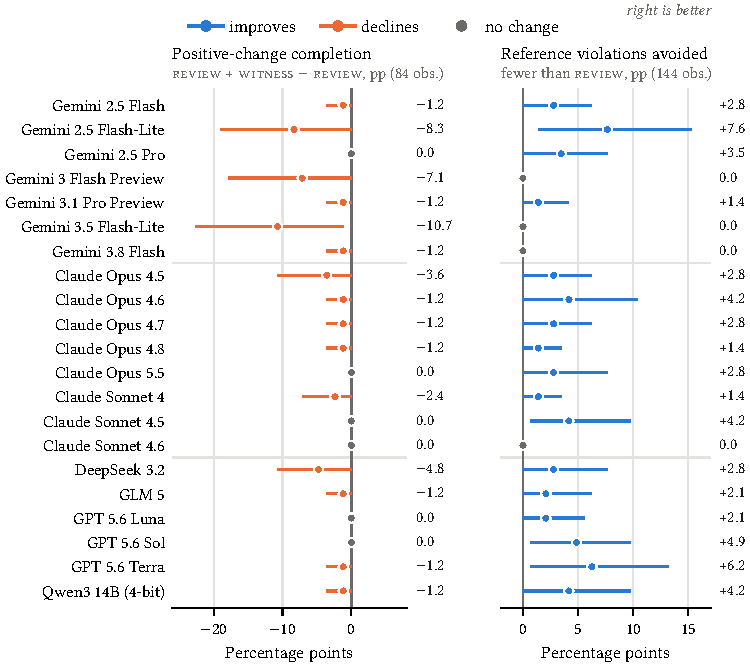
\includegraphics[width=\linewidth,height=.58\textheight,keepaspectratio]{media/figure_09.pdf}
\caption{\review{} + \witness{} minus \review{}, oriented so that improvement is to the right. Blue marks improvement, orange decline and gray no change; values at the right are point estimates in percentage points. Intervals cluster the three repetitions within each original case and are exploratory pointwise intervals. Both favorable restraint and unfavorable completion effects are shown.}\label{fig:L1}
\Description{\review{} + \witness{} minus \review{}, oriented so that improvement is to the right. Intervals cluster the three repetitions within each original case and are exploratory pointwise intervals. Both favorable restraint and unfavorable completion effects are shown.}
\end{figure}

\subsection{Variant Audit of the 82 Avoided Reference Violations}
Section~6.4 asks which of the 82 reference-violating states that \review{}+\witness{} avoids relative to \review{} are semantic errors under the reference and which are representational mismatches. The audit uses only archived artifacts. For each of the 82 paired observations, we took the reference components that the \review{} state failed from the saved scores and the held operation from the saved gate log of the hybrid. For each case, we collected the facts that are new relative to the initial state in every replayed output whose executed state conforms to the reference; in each affected positive case, all conforming states contain the same single new fact, the required fact. A held append counts as a \emph{variant} of that fact when it has the same relation and time and one of the following holds after Unicode NFC, case folding, and whitespace removal: subject and value are equal although the raw strings differ (spacing); the values are equal and one subject string contains the other or both denote the participant (``participant'' or ``p1''; subject label); or one value contains the other and the subjects match in the same sense (value form).

The rule was written after the avoided observations had been listed and is applied mechanically; it is not a semantic judgment, and no person rated the outputs. It undercounts variants that need translation or restructuring, such as ``email'' for ``이메일'' or a subject that names the farm rather than the participant. Table~\ref{tab:L9} gives the result. Each of the 71 append observations contains exactly one held append, and in all 52 variant observations the required fact is absent under both \review{} and the hybrid, so positive-change completion fails either way.

\begin{table}[H]
\centering
\caption{Composition of the 82 reference-violating states avoided by \review{}+\witness{} relative to \review{} (observations; 21 configurations, three repetitions). ``Forbidden'' means that the \review{} state contains a tuple the reference forbids; all other append holds failed only because of an unlisted fact. English glosses are translations.}\label{tab:L9}
\small
\setlength{\tabcolsep}{3pt}
\begin{tabular}{@{}>{\raggedright\arraybackslash}p{\dimexpr0.2000\linewidth-6pt\relax}>{\raggedright\arraybackslash}p{\dimexpr0.3000\linewidth-6pt\relax}>{\raggedright\arraybackslash}p{\dimexpr0.3600\linewidth-6pt\relax}r@{}}
\toprule
\textbf{Class (cases)} & \textbf{Required fact} & \textbf{Held tuple} & \textbf{Obs.} \\
\midrule
\multicolumn{4}{@{}l}{\emph{Append holds, variants of a required fact (52 observations, nine cases)}} \\
Subject label (CT13) & 준호 $\cdot$ hobby $\cdot$ 낚시 & 남편 준호 (``husband Junho''), participant의 남편 준호 & 10 \\
Subject label (CT14) & 순자 $\cdot$ birthplace $\cdot$ 임실 & 어머니 순자 (``mother Sunja''), participant의 어머니 순자 & 3 \\
Subject label (CT15) & 도윤 $\cdot$ workplace $\cdot$ 대한우편 & 아들 도윤 (``son Doyun''), participant의 아들 도윤 & 7 \\
Subject label (CT16) & 영숙 $\cdot$ learned\_from $\cdot$ 이 사범님 & 동생 영숙 (``sibling Youngsook''), participant의 동생 영숙 & 8 \\
Subject label (CT27) & participant $\cdot$ shop\_name $\cdot$ 장미미용실 & subject p1 & 1 \\
Spacing (CT20) & participant $\cdot$ hobby $\cdot$ 우표수집 & 우표 수집 (``stamp collecting'') & 6 \\
Value form (CT31) & participant $\cdot$ event\_year $\cdot$ 2003년 & 2003; 서안농장 개업 2003년 and similar & 11 \\
Value form (CT44) & participant $\cdot$ hobby $\cdot$ 자전거 & 자전거 타기 (``riding a bicycle'') & 5 \\
Value form (CT26) & participant $\cdot$ learned\_from $\cdot$ 오 선생님 & 기타: 오 선생님 & 1 \\
\addlinespace[2pt]
\multicolumn{4}{@{}l}{\emph{Other append holds (19 observations)}} \\
Unlisted fact (CT16, CT24, CT26, CT29, CT31, CT39) & -- & e.g., another teacher's name; email for 이메일; the farm as subject; subject and value swapped & 17 \\
Forbidden (CT23) & -- & a destination on which the readings disagree (Qwen3 14B) & 2 \\
\addlinespace[2pt]
\multicolumn{4}{@{}l}{\emph{Correction holds (11 observations)}} \\
Forbidden (CT11, CT21, CT22) & -- & overwrite of a protected record with a forbidden value & 11 \\
\bottomrule
\end{tabular}
\end{table}

The audit changes the reading of Table~\ref{tab:L4}, not its counts. Of the 71 violations avoided by APPEND holds, 52 come from withholding a required fact written in another form, and 19 from withholding a fact that no conforming state contains; the 11 avoided by CORRECT holds all involve a forbidden value.
\FloatBarrier
\setcounter{figure}{0}\setcounter{table}{0}
\renewcommand{\thefigure}{J\arabic{figure}}
\renewcommand{\thetable}{J\arabic{table}}
\section{Follow-Up Runs}
The runs in this appendix were collected after the results of the main article had been inspected, as tests of its diagnoses (main article, Sections~5.1, 6.1, 6.6, and 6.7). Each had a frozen contract that fixed the selection, prompts, structural schemas, comparisons, stopping rules, and analysis before any output. Each ran once, with no retry or repair; an invalid output counts as a system failure, and an unreturned call leaves its case out of that model's paired denominator rather than scoring it as zero. No model was trained, and no archived score was recomputed or overwritten. On the main cases, the reference is the authored specification of the main article; on DSTC2, it derives from the corpus labels. All paired intervals are 95\% percentile intervals from 5,000 cluster bootstrap draws with seed 20261004, clustering by case on the main cases and by caller on DSTC2.

\subsection{Revised Extraction Instruction}
The comparison holds the saved controlled-path proposal, the \agree{} gate, the executor, and the reference fixed and varies only the extraction instruction. The revised instruction, written once before any response and not tuned afterward, adds the following paragraph to the original extraction prompt (translated from Korean): ``Record extraction locations explicitly. An atomic fact that a reading explicitly confirms after a correction must also be recorded in that reading's facts; do not omit it from the facts because the correction evidence is recorded in the correction witnesses. Record the corrected new value with the existing subject, relation, and time in the fact schema. Do not record negated, uncertain, or other people's facts as confirmed facts of the existing person. Do not copy a fact supported by only one reading into another reading's facts. Do not add facts absent from the source.''

Gemini 2.5 Flash used temperature 0.2 and a thinking budget of 0, and Gemini 3.8 Flash temperature 0.2 and the LOW thinking level; both had an output cap of 8,192 tokens. For each of the five Gemini 2.5 Flash cases with extraction-induced holds, the selected repetition is the earliest one in which \agree{} held the correction; each case received one new response under each instruction (Table~\ref{tab:M1}). Under the original instruction, the four reproduced holds again show the pattern of the main article's Section~6.1: both fact lists are empty, and every reading carries an affirmed witness for the corrected value. Under the revised instruction, the witnesses are unchanged and the corrected tuple appears in both fact lists.

\begin{table}[H]
\centering
\caption{Re-extraction of the five Gemini 2.5 Flash cases, one new response per instruction, gated by the unchanged \agree{} rule on the saved proposal. ``Shared'' means that the corrected tuple is in the fact lists of both readings. No output in either arm produced a reference-violating state.}\label{tab:M1}
\small
\setlength{\tabcolsep}{3pt}
\begin{tabular}{@{}l>{\raggedright\arraybackslash}p{0.34\linewidth}c>{\raggedright\arraybackslash}p{0.17\linewidth}>{\raggedright\arraybackslash}p{0.17\linewidth}@{}}
\toprule
\textbf{Case} & \textbf{Proposed correction} & \textbf{Rep.} & \textbf{Original: shared / completed} & \textbf{Revised: shared / completed} \\
\midrule
CT01 & birthplace $\leftarrow$ 대구 (Daegu) & 1 & yes / yes & yes / yes \\
CT42 & birthplace $\leftarrow$ 문경 (Mungyeong) & 3 & no / no & yes / yes \\
CT45 & event\_year $\leftarrow$ 1993년 & 1 & no / no & yes / yes \\
CT46 & learned\_from $\leftarrow$ 신 선생님 (teacher Shin) & 1 & no / no & yes / yes \\
CT48 & meeting\_place $\leftarrow$ 시민운동장 (civic stadium) & 1 & no / no & yes / yes \\
\addlinespace[2pt]
Total & & & 1 / 1 of 5 & 5 / 5 of 5 \\
\bottomrule
\end{tabular}
\end{table}

CT01 recovered spontaneously under the original instruction and is therefore not counted as an effect of the revision. On Gemini 3.8 Flash, both instructions were applied to the saved controlled-path proposal of repetition~1 for all 48 cases. The outcomes are identical case by case: 11 of 11 strict corrections, 27 of 28 positive changes, 47 of 48 conforming states, and no reference violation under either instruction. A planned comparison on all 48 Gemini 2.5 Flash cases stopped at a provider error after 23 original-instruction and 27 revised-instruction extractions and is not analyzed; the five pairs in Table~\ref{tab:M1} were completed in two later collections, one of which stopped at a rate-limit error and was completed by a three-request recovery. Four of the ten responses in the table come from the stopped collection.

\subsection{Learned Verifier}
The verifier (Gemini 3.1 Pro Preview, temperature 0.2, LOW thinking level, output cap 8,192 tokens) received the public case (context, all readings, initial memory, and retention permission) and the indexed list of proposed APPEND and CORRECT operations of one saved \review{} proposal, and returned, in a fixed JSON schema, one decision per operation: an approval flag and a short reason. A disapproved operation becomes HOLD; nothing else in the proposal changes, and the result is executed with the frozen executor and scored with the archived evaluator. The verifier saw neither the extraction, the reference, nor any earlier gate decision. Its instruction reads (translated from Korean): ``You verify memory writes in a personal conversation. For each APPEND or CORRECT proposal, judge whether the write is justified, considering all candidate transcripts, the dialogue context, the existing memory, and storage consent together. The transcript alternatives are possible readings of the same utterance, and the write needs support in all of them. Accept equivalent meanings that differ only in wording. Distinguish other people's information, differences in time, negation, uncertainty, and quotation from actual assertion. For CORRECT, check that it truly corrects the designated existing record; if there is an explicit correction, do not reject it only because it differs from the past value. Do not approve when storage consent is denied or unknown. No reference, earlier policy decision, or answer is provided, and the proposals may be wrong.''

The selected proposals are repetition~1 of every case for Gemini 3.8 Flash and Qwen3 14B and for Gemini 2.5 Flash, except CT42, for which repetition~3 holds the correction (Table~\ref{tab:M1}); the deterministic conditions are the archived scores for the same repetitions. All 144 calls returned valid decisions. The verifier held 4 of 15 proposed corrections and none of 17 appends on Gemini 2.5 Flash, nothing among 11 corrections and 17 appends on Gemini 3.8 Flash, and 7 of 18 corrections and 6 of 20 appends on Qwen3 14B (Table~\ref{tab:M2}). The calls had a mean latency of 4.39 seconds (median 3.58) and used on average 673 input, 35 output, and 144 reasoning tokens.

\begin{table}[H]
\centering
\caption{All conditions on the same saved \review{} proposals, one repetition per case. Denominators are 11 correction, 28 positive, and 48 cases for reference-violating and conforming states.}\label{tab:M2}
\small
\setlength{\tabcolsep}{3pt}
\begin{tabular}{@{}llrrrr@{}}
\toprule
\textbf{Configuration} & \textbf{Condition} & \textbf{Correct. /11} & \textbf{Positive /28} & \textbf{Viol. /48} & \textbf{Conform. /48} \\
\midrule
Gemini 2.5 Flash & \review{} & 11 & 27 & 2 & 46 \\
 & \review{} + \agree{} & 6 & 22 & 1 & 42 \\
 & \review{} + \allow{} & 11 & 27 & 2 & 46 \\
 & \review{} + \literal{} & 11 & 27 & 1 & 47 \\
 & \review{} + \witness{} & 11 & 27 & 1 & 47 \\
 & \review{} + verifier & 11 & 27 & 1 & 47 \\
\addlinespace[2pt]
Gemini 3.8 Flash & \review{} & 11 & 28 & 0 & 48 \\
 & \review{} + any of the four rules & 11 & 27 & 0 & 47 \\
 & \review{} + verifier & 11 & 28 & 0 & 48 \\
\addlinespace[2pt]
Qwen3 14B (4-bit) & \review{} & 11 & 24 & 4 & 42 \\
 & \review{} + any of the four rules & 11 & 24 & 3 & 43 \\
 & \review{} + verifier & 11 & 24 & 1 & 44 \\
\bottomrule
\end{tabular}
\end{table}

Relative to \review{}+\witness{}, the verifier differs only on Gemini 3.8 Flash (positive changes $+3.57$ percentage points, interval 0.00 to 10.71; conformity $+2.08$, 0.00 to 6.25) and Qwen3 14B (reference violations $-4.17$, $-10.42$ to 0.00; conformity $+2.08$, 0.00 to 6.25). Relative to \review{}+\agree{} on Gemini 2.5 Flash, it completes five more corrections ($+45.5$ points, 18.2 to 72.7), the same five that \allow{}, \literal{}, and \witness{} release. On Gemini 2.5 Flash, one of its held corrections, in the conflicting-transcript case CT21, reproduces the \review{}+\witness{} hold; the other three leave every endpoint as under \review{}. The three state differences from \review{}+\witness{} are described in the main article's Section~6.6.

\subsection{Real Speech-Recognition Hypotheses (DSTC2)}
\paragraph{Source and selection.} The source is the official DSTC2 test release (\url{https://github.com/matthen/dstc}). One user turn was taken from each of 48 distinct dialogues, from 41 callers, by a hash-ranked rule with a fixed seed applied before any model output: 24 goal revisions, 12 denials without an explicit replacement, and 12 reference-enriched n-best turns whose recognition errors were identified with the labels, which form a separately reported diagnostic stratum. The sample serves diagnosis and does not estimate how often such turns occur.

\paragraph{Input and reference.} The readings are all distinct non-empty strings of the live 10-best list in their original rank order (433 over the 48 turns); exact duplicates and blank strings are omitted without rewriting, and no likelihood weight is used. The history consists of the earlier system turns and top-ranked user hypotheses, and the previous official goal for food, area, and price range seeds the memory; the current transcript and labels are withheld. The domain adapter replaces the Korean personal relations with these three slots and leaves the gate logic unchanged; retention permission is set to allowed as a task fixture, not as observed consent. The reference is the official goal derived from human-reviewed semantic labels, compared as exact lowercase values without normalization. Goal conformity requires all three slots to match; a new wrong write introduces a slot value absent from the official goal, whereas a stale prior value fails goal conformity without counting as a new wrong write; required-change completion counts turns whose goal changes. Actions and consent are not scored. DELETE is not supported by the adapter, and no selected turn required removing a slot.

\paragraph{Collection.} Gemini 3.1 Pro Preview and Gemini 3.8 Flash ran with temperature 0.2, the LOW thinking level, an output cap of 8,192 tokens, and one repetition. A model stopped at its first transport or provider failure. Gemini 3.1 Pro Preview completed all 48 turns; Gemini 3.8 Flash stopped after 22 valid turns (21 callers), with no denial turn among them. The 142 attempts produced 70 valid pairs. The two models are not pooled.

\begin{table}[H]
\centering
\caption{DSTC2 outcomes by stratum, as goal conformity / required changes completed / new wrong writes. ``Ungated'' executes the proposal without admission. Gemini 3.8 Flash is a partial run and is not pooled with Gemini 3.1 Pro Preview.}\label{tab:M3}
\small
\setlength{\tabcolsep}{3pt}
\begin{tabular}{@{}llllll@{}}
\toprule
\textbf{Model and stratum (turns)} & \textbf{Ungated} & \textbf{\allow{}} & \textbf{\agree{}} & \textbf{\literal{}} & \textbf{\witness{}} \\
\midrule
\multicolumn{6}{@{}l}{\textit{Gemini 3.1 Pro Preview}} \\
Goal revision (24) & 20 / 20 / 1 & 20 / 20 / 1 & 5 / 5 / 0 & 5 / 5 / 0 & 5 / 5 / 0 \\
Denial (12; 1 change) & 10 / 1 / 2 & 10 / 1 / 2 & 12 / 1 / 0 & 11 / 1 / 1 & 12 / 1 / 0 \\
Recognition error (12; 11 changes) & 3 / 2 / 0 & 3 / 2 / 0 & 1 / 0 / 0 & 1 / 0 / 0 & 1 / 0 / 0 \\
All (48; 36 changes) & 33 / 23 / 3 & 33 / 23 / 3 & 18 / 6 / 0 & 17 / 6 / 1 & 18 / 6 / 0 \\
\addlinespace[2pt]
\multicolumn{6}{@{}l}{\textit{Gemini 3.8 Flash, partial}} \\
All valid (22; 21 changes) & 9 / 8 / 1 & 9 / 8 / 1 & 3 / 2 / 0 & 3 / 2 / 0 & 3 / 2 / 0 \\
\bottomrule
\end{tabular}
\end{table}

\paragraph{Holds and paired comparisons.} On Gemini 3.1 Pro Preview, \agree{} held a proposed correction in 20 outputs (16 goal revisions, two denials, and two recognition-error turns) and held no append. Ten holds arise from different values extracted from different hypotheses and ten from a value supported by only some hypotheses or omitted from some; none shows the extraction pattern of the main source. \allow{} releases all 20: 17 complete a required change and three introduce a wrong value (DSTC2\_17, DSTC2\_40, and DSTC2\_45). \literal{} releases only DSTC2\_45, a wrong write, and \witness{} releases none. Relative to \allow{}, \witness{} changes goal conformity by $-31.25$ percentage points (caller-cluster interval $-45.83$ to $-16.33$), required-change completion by $-47.22$ ($-62.86$ to $-32.26$; 36 turns from 31 callers), and turns with a new wrong write by $-6.25$ ($-13.46$ to 0.00); \literal{} changes them by $-33.33$ ($-47.73$ to $-19.23$), $-47.22$, and $-4.17$ ($-10.42$ to 0.00). On the partial Gemini 3.8 Flash run, \agree{} held seven corrections, six for partial support or omission and one for different values.

\paragraph{Data terms.} DSTC2 is used under its own terms. The archive contains no corpus text, transcript-bearing input, gold value, or model response derived from it; it provides the selected dialogue paths, turn indices, and source hashes, the adapter and evaluation code that reconstruct the 48 inputs from an independently obtained copy, and scalar outcome flags with pseudonymized caller clusters that reproduce the tables and intervals.

\subsection{Korean Memory-Operation Data}
The Korean memory-operation data of Bae et al.\ (main article, reference on memory management in long-term conversations) would supply a human-labeled reference for the specification confound. The official public repository we inspected contains Korean samples and machine-translated English material, but not the original operation-label pairs, example identifiers, session links, or official split files that a replication requires. No model call or evaluation was therefore made on this source. Its REPLACE operations also include changes over time and added detail, so not every REPLACE is a correction of an earlier error.
\FloatBarrier
\setcounter{figure}{0}\setcounter{table}{0}
\renewcommand{\thefigure}{K\arabic{figure}}
\renewcommand{\thetable}{K\arabic{table}}
\section{Variant-Tolerant Re-Scoring}
\subsection{Definition and Implementation}
The variant-tolerant reference re-scores the saved final states; it executes no policy and calls no model. A final tuple $f$ matches a reference tuple $r$ when $f=r$, or when relation and time are equal, the subjects match, and the values match. After Unicode NFC, case folding, and removal of all whitespace, subjects match when they are equal, when both are participant labels (\texttt{participant} or \texttt{p1}), or when one contains the other and neither is a participant label; values match when they are equal or one contains the other. A required tuple is present when some final tuple matches it, a final tuple that matches a required tuple is not an extra fact, and a protected record is preserved when its final tuple matches its initial tuple. Forbidden tuples, obsolete versions, removals, actions, and validity are scored exactly as before, so the second reference can only credit an output. The scorer wraps the archived evaluator: with matching switched off, it reproduces every score field except the call-identifier string in all 42,336 archived condition rows of the panel (3,024 episodes, 14 conditions), and the reference-violation and correction fields of the 1,152 archived controlled-path \allow{} rows. The rule was written after the variant audit of Online Appendix~I and is broader than that audit only in applying to every final tuple rather than to held appends. The scripts are in the archive under \texttt{analysis\_v29}.

Table~\ref{tab:K1} lists every pair that the rule accepts. Each accepted pair restates the required fact with a kinship label, an underscore or possessive form of the same subject, the speaker identifier \texttt{p1} for the participant, a spacing difference, the year without its counter suffix (2003 for 2003년), or additional words around the same value. No forbidden tuple is affected, because forbidden tuples are not relaxed.

\begin{table}[H]
\centering
\caption{All 38 surface-variant pairs accepted by the variant-tolerant reference, grouped by case. The third column shows the differing subject or value of each accepted tuple and, in parentheses, the number of condition-level observations among the 42,336 scored rows in which it occurs. English glosses: 남편 husband, 어머니 mother, 아들 son, 동생 younger sibling, 기타 guitar, 개업 opening, 타기 riding.}\label{tab:K1}
\footnotesize
\setlength{\tabcolsep}{3pt}
\begin{tabular}{@{}l>{\raggedright\arraybackslash}p{0.30\linewidth}>{\raggedright\arraybackslash}p{0.56\linewidth}@{}}
\toprule
\textbf{Case} & \textbf{Required fact} & \textbf{Accepted forms (observations)} \\
\midrule
CT13 & 준호 $\cdot$ hobby $\cdot$ 낚시 & 남편 준호 (36); participant의 남편 준호 (27); 남편\_준호 (1); participant\_spouse(준호) (1); 준호 (participant의 남편) (1); participant\_spouse\_준호 (1) \\
CT14 & 순자 $\cdot$ birthplace $\cdot$ 임실 & 어머니 순자 (215); participant의 어머니 순자 (29); participant's mother 순자 (7); 순자(어머니) (2); participant\_mother\_순자 (1); 순자(participant의 어머니) (1) \\
CT15 & 도윤 $\cdot$ workplace $\cdot$ 대한우편 & 아들 도윤 (75); participant의 아들 도윤 (16); participant\_son\_도윤 (2); 아들\_도윤 (1) \\
CT16 & 영숙 $\cdot$ learned\_from $\cdot$ 이 사범님 & 동생 영숙 (95); participant의 동생 영숙 (15); participant\_sibling:영숙 (1); participant\_sibling\_영숙 (1); 영숙(p1 동생) (1); participant.younger\_sibling.영숙 (1) \\
CT20 & participant $\cdot$ hobby $\cdot$ 우표수집 & 우표 수집 (29) \\
CT26 & participant $\cdot$ learned\_from $\cdot$ 오 선생님 & 오 선생님 (기타) (4); 기타: 오 선생님 (4); 기타:오 선생님 (2); 오 선생님(기타) (1); 기타 - 오 선생님 (1) \\
CT27 & participant $\cdot$ shop\_name $\cdot$ 장미미용실 & p1 (115) \\
CT30 & participant $\cdot$ travel\_destination $\cdot$ 여수 & p1 (12) \\
CT31 & participant $\cdot$ event\_year $\cdot$ 2003년 & 2003 (348); 서안농장 개업 2003년 (11); 농장 개업 2003년 (3); 서안농장 개업: 2003년 (3); 2003년 서안농장 개업 (2); 농장을 처음 연 해는 2003년 (2); 2003년 농장 개업 (1) \\
CT44 & participant $\cdot$ hobby $\cdot$ 자전거 & 자전거 타기 (10) \\
\bottomrule
\end{tabular}
\end{table}

\subsection{Rule Comparisons and Configurations}
Table~\ref{tab:K2} repeats main-article Table~6 with Qwen3 14B and adds the violation counts under the variant-tolerant reference. Strict correction counts are identical under both references, and every difference between two rules is the same; only the level of the violation counts falls. Across the full panel, controlled-path strict corrections are 673, 685, and 685 under \agree{}, \literal{}, and \witness{} under both references, and violations fall from 131, 133, and 131 to 54, 56, and 54. On the 36 controlled-path outputs and the 23 review-proposal outputs on which at least two of the four rules produce different endpoints, every pairwise output-level difference is the same under both references. By contrast, \review{} and \review{}+\witness{} produce different endpoints on 127 outputs, and their difference changes with the reference on 52; the controlled path and \review{} differ on 199 outputs, and on 61 the difference changes.

\begin{table}[H]
\centering
\caption{Rules on identical controlled-path proposals, in the order \agree{} / \allow{} / \literal{} / \witness{}, three repetitions. Strict correction is over 33 observations and reference-violating states over 144.}\label{tab:K2}
\small
\setlength{\tabcolsep}{3pt}
\begin{tabular}{@{}llll@{}}
\toprule
\textbf{Configuration} & \textbf{Correction (both)} & \textbf{Viol., exact} & \textbf{Viol., variant-tolerant} \\
\midrule
Gemini 2.5 Flash & 22 / 33 / 33 / 33 & 3 / 3 / 3 / 3 & 2 / 2 / 2 / 2 \\
Gemini 2.5 Pro & 31 / 31 / 31 / 31 & 3 / 9 / 4 / 3 & 0 / 6 / 1 / 0 \\
Gemini 2.5 Flash-Lite & 31 / 31 / 31 / 31 & 16 / 19 / 16 / 16 & 10 / 13 / 10 / 10 \\
Gemini 3 Flash Preview & 33 / 33 / 33 / 33 & 12 / 12 / 12 / 12 & 9 / 9 / 9 / 9 \\
Gemini 3.1 Pro Preview & 33 / 33 / 33 / 33 & 2 / 2 / 2 / 2 & 1 / 1 / 1 / 1 \\
Gemini 3.5 Flash-Lite & 32 / 32 / 32 / 32 & 7 / 12 / 7 / 7 & 4 / 9 / 4 / 4 \\
Gemini 3.8 Flash & 33 / 33 / 33 / 33 & 1 / 1 / 1 / 1 & 0 / 0 / 0 / 0 \\
Qwen3 14B (4-bit) & 33 / 33 / 33 / 33 & 20 / 29 / 20 / 20 & 17 / 26 / 17 / 17 \\
\bottomrule
\end{tabular}
\end{table}

Table~\ref{tab:K3} gives every panel configuration in the order \review{} / \review{}+\witness{} / controlled path. Under the exact reference these are the counts of Tables~G1 and I8; under the variant-tolerant reference, \review{} has no reference-violating state on 10 configurations, so the gate prevents nothing there while it still holds appends.

\begin{table}[H]
\centering
\caption{All 21 configurations under both references, in the order \review{} / \review{}+\witness{} / controlled path. Reference violations are over 144 observations and positive changes over 84.}\label{tab:K3}
\small
\setlength{\tabcolsep}{3pt}
\begin{tabular}{@{}lllll@{}}
\toprule
 & \multicolumn{2}{c}{\textbf{Viol. /144 $\downarrow$}} & \multicolumn{2}{c}{\textbf{Positive /84 $\uparrow$}} \\
\cmidrule(lr){2-3}\cmidrule(l){4-5}
\textbf{Configuration} & \textbf{Exact} & \textbf{Variant-tol.} & \textbf{Exact} & \textbf{Variant-tol.} \\
\midrule
Claude Opus 4.5 & 5 / 1 / 6 & 0 / 0 / 3 & 79 / 76 / 78 & 84 / 77 / 81 \\
Claude Opus 4.6 & 8 / 2 / 6 & 2 / 2 / 4 & 76 / 75 / 78 & 82 / 75 / 80 \\
Claude Opus 4.7 & 6 / 2 / 3 & 0 / 0 / 0 & 78 / 77 / 80 & 84 / 79 / 83 \\
Claude Opus 4.8 & 3 / 1 / 2 & 0 / 0 / 0 & 81 / 80 / 82 & 84 / 81 / 84 \\
Claude Opus 5.5 & 15 / 11 / 12 & 0 / 0 / 0 & 69 / 69 / 72 & 84 / 80 / 84 \\
Claude Sonnet 4 & 6 / 4 / 6 & 1 / 0 / 0 & 77 / 75 / 76 & 82 / 79 / 82 \\
Claude Sonnet 4.5 & 9 / 3 / 3 & 4 / 0 / 0 & 79 / 79 / 81 & 84 / 82 / 84 \\
Claude Sonnet 4.6 & 3 / 3 / 3 & 0 / 0 / 0 & 81 / 81 / 81 & 84 / 84 / 84 \\
DeepSeek 3.2 & 5 / 1 / 7 & 4 / 0 / 3 & 81 / 77 / 76 & 82 / 78 / 80 \\
GLM 5 & 3 / 0 / 2 & 0 / 0 / 0 & 81 / 80 / 81 & 84 / 80 / 83 \\
GPT 5.6 Luna & 7 / 4 / 4 & 0 / 0 / 0 & 77 / 77 / 80 & 84 / 81 / 84 \\
GPT 5.6 Sol & 13 / 6 / 8 & 0 / 0 / 0 & 71 / 71 / 75 & 84 / 77 / 83 \\
GPT 5.6 Terra & 13 / 4 / 5 & 1 / 0 / 1 & 71 / 70 / 76 & 83 / 74 / 80 \\
Gemini 2.5 Flash & 5 / 1 / 3 & 3 / 0 / 2 & 82 / 81 / 80 & 84 / 82 / 81 \\
Gemini 2.5 Flash-Lite & 14 / 3 / 16 & 8 / 0 / 10 & 69 / 62 / 56 & 75 / 65 / 62 \\
Gemini 2.5 Pro & 8 / 3 / 3 & 1 / 0 / 0 & 71 / 71 / 73 & 78 / 74 / 76 \\
Gemini 3 Flash Preview & 6 / 6 / 12 & 6 / 6 / 9 & 78 / 72 / 71 & 78 / 72 / 74 \\
Gemini 3.1 Pro Preview & 3 / 1 / 2 & 3 / 1 / 1 & 81 / 80 / 81 & 81 / 80 / 82 \\
Gemini 3.5 Flash-Lite & 0 / 0 / 7 & 0 / 0 / 4 & 84 / 75 / 74 & 84 / 75 / 77 \\
Gemini 3.8 Flash & 0 / 0 / 1 & 0 / 0 / 0 & 84 / 83 / 83 & 84 / 83 / 84 \\
Qwen3 14B (4-bit) & 14 / 8 / 20 & 11 / 5 / 17 & 73 / 72 / 66 & 76 / 75 / 69 \\
\bottomrule
\end{tabular}
\end{table}

\subsection{Decomposition and Intervals}
The decomposition of main-article Table~8 is an identity on paired observations: for each configuration, case, and repetition, the controlled path minus \review{} equals the controlled path minus \review{}+\witness{} plus \review{}+\witness{} minus \review{}. The two left-hand conditions share the extraction and the \witness{} gate and differ only in the proposal; the gate term is attributed to the held operation recorded in the saved gate log, and to invalid extraction when the hybrid output is invalid. No paired observation changed through both a held APPEND and a held CORRECT. Table~\ref{tab:K4} gives pooled paired differences with 95\% case-cluster percentile intervals (5,000 draws, seed 20261005, keeping all configurations and repetitions of a case together). Because the seed differs from the archived analyses, the exact-reference gate intervals differ slightly from those of Online Appendix~I.

\begin{table}[H]
\centering
\caption{Pooled paired differences in percentage points with 95\% case-cluster intervals over 48 (violations, conformity) or 28 (positive changes) case clusters.}\label{tab:K4}
\footnotesize
\setlength{\tabcolsep}{3pt}
\begin{tabular}{@{}>{\raggedright\arraybackslash}p{0.34\linewidth}lll@{}}
\toprule
\textbf{Contrast and reference} & \textbf{Viol.\,$\downarrow$} & \textbf{Positive\,$\uparrow$} & \textbf{Conformity\,$\uparrow$} \\
\midrule
Proposal: controlled path $-$ \review{}+\witness{}, exact & $+2.22$ [$+1.03$, $+3.67$] & $+0.96$ [$-0.79$, $+2.72$] & $+0.56$ [$-0.63$, $+1.79$] \\
Proposal: controlled path $-$ \review{}+\witness{}, variant-tolerant & $+1.32$ [$+0.56$, $+2.22$] & $+2.49$ [$-0.11$, $+5.44$] & $+1.46$ [$-0.26$, $+3.37$] \\
Gate: \review{}+\witness{} $-$ \review{}, exact & $-2.71$ [$-4.33$, $-1.36$] & $-2.27$ [$-4.08$, $-0.85$] & $-0.89$ [$-2.15$, $+0.26$] \\
Gate: \review{}+\witness{} $-$ \review{}, variant-tolerant & $-0.99$ [$-1.69$, $-0.40$] & $-5.22$ [$-8.22$, $-2.49$] & $-2.61$ [$-4.79$, $-0.73$] \\
Complete pipeline: controlled path $-$ \review{}, exact & $-0.50$ [$-1.92$, $+0.93$] & $-1.30$ [$-3.40$, $+0.79$] & $-0.33$ [$-1.88$, $+1.26$] \\
Complete pipeline: controlled path $-$ \review{}, variant-tolerant & $+0.33$ [$-0.66$, $+1.32$] & $-2.72$ [$-4.59$, $-1.02$] & $-1.16$ [$-2.68$, $+0.40$] \\
\bottomrule
\end{tabular}
\end{table}
\FloatBarrier
\end{document}
